\documentclass[twoside,english]{uiofysmaster}
\usepackage[english]{babel}
\usepackage{tikz}
\usepackage{amsmath}
\usepackage[version=4]{mhchem}
\usepackage{float}
\usepackage{mathtools}
\usepackage[ruled,vlined]{algorithm2e}
\usepackage{hyperref}
\usepackage{enumerate}
\usepackage[shortlabels]{enumitem}
\usepackage{amssymb}
\usepackage{subfig}
\usepackage{makecell}
\usepackage{array}
\usepackage{multirow}
\usepackage{mathpazo}
\usepackage{siunitx}
\usepackage{graphicx}
\usepackage{longtable}
\usepackage[toc,page]{appendix}
\usepackage{booktabs}
\usepackage{tabularx}
\usepackage{adjustbox}
\usepackage[section]{placeins}
\usepackage{pdflscape}
\usepackage[utf8]{inputenc}
\usepackage[T1]{fontenc}

% custom commands
\newcommand{\colorlinks}[2]{{\hypersetup{allcolors=#1}#2}}
\newcommand{\bs}[1]{{\boldsymbol{#1}}}
\newcommand{\ddx}[1]{{\frac{\partial #1}{\partial x}}}
\newcommand{\dd}[2]{{\frac{\partial #1}{\partial #2}}}

%\bibliography{references}
\usepackage[numbers]{natbib}

\author{Geir Tore Ulvik}
\title{Supervised Learning in a Low-Energy Nuclear Physics Experiment}
\date{January 2020}
\begin{document}
\maketitle

\tableofcontents
\listoffigures

\newpage
\section*{Acknowledgements}
Acknowledgement text like lorem ipsum all up in here.
\newpage


\begin{abstract}
    This is the abstract text.
\end{abstract}

\chapter{Introduction}
\noindent In this thesis, we approach the problem arising from copious amounts of unlabeled data
generated in nuclear physics experiments. Modelling the world around us to predict behaviour and increase 
our understanding is a key concept in physics, and science as a whole. Simulating physical processes often 
lay the groundwork for verifying theory, and designing experiments. For many branches of physics, 
and especially nuclear physics, there has been an exponential growth in data generated from experiments. 
This brings several challenges, the most immediate of which may be "how do we process it all?". If there are 
multiple types of
reactions occurring in an experiment, how can we separate them when there are billions of events?
In the later years, machine learning algorithms have gained popularity for accomplishing this task,
alleviating the need for humans to sift through vast amounts of data by hand. 
Machine learning has already been used in a wide variety of applications, such as at CERN \ref{Arpaia2021},
and the Active-Target Time Projection Chamber (AT-TPC) at the National Superconducting Cyclotron Laboratory
at Michigan State University \ref{Kuchera2019}. In this thesis, we explore the leveraging of simulated experiments to train machine learning models and subsequently
apply them to data gathered from real-world experiments.


\noindent In simulations, we have complete knowledge of every parameter. The energy of a decay, the exact positions
of the ion where the decay originated, the exact time of the decay are all examples of knowledge we have about
simulations. For experimental data, these details are what we seek to learn in order to verify and improve our
model of the physical universe, and they are not necessarily directly measurable.
Traditional methods of analysis may be computationally expensive to run, especially considering the
amounts of data these methods must churn through, with repeated calculations for every sample.
With machine learning algorithms we can front-load all these computations, training them to perform
the task of extracting our desired information based on simulations. If our simulations capture crucial
attributes of the real data, we may be able to approximate even values that would be notoriously difficult 
to measure or infer from data alone. Another avenue is determining the types of reactions or events that
occur in experimental data. This is of particular interest in this specific case, as there is currently no methods
other than the human eye to separate events into their respective categories. 

\noindent We investigate the possibility of carrying out three different tasks. Classification, prediction of event energy, and prediction of
positions of origin. We introduce the fundamental concepts for machine learning theory, our methods and
implementation, and present results of carrying our these tasks on simulated and experimental data.
\chapter{Theory}
In this thesis we explore the use of supervised learning on simulated and experimental
nuclear physics data. To build a foundation for the following discussion, we introduce
the fundamental concepts underpinning the advanced machine learning techniques of
today.

We note that the following chapter follows closely the work of 
Morten Hjorth-Jensen\cite{mhjensen-fys4155-notes}, Mehta et. al\cite{Mehta2019},
Goodfellow et. al\cite{Goodfellow-et-al-2016}, and the University of Stanfords
course CS231n\cite{cs231n}.
\section{Linear Regression}\label{sec:linreg}
Suppose you have a data set $\mathcal{L}$ consisting of the data
$\mathbf{X}_\mathcal{L}=\{(y_i, x_i), i=0\ldots n-1\}$. Each point is associated
with a scalar target $y_i$, and a vector $\bs{x}$ containing values for $p$ input
features. Assuming the target variable $y_i$ is linear in the inputs, it can be
written as a linear function of the features, given by
\begin{equation}\label{eq:ols-target}
y_i = w_0 x_{i,0} + w_1 x_{i,1} + ... + w_{p-1} x_{i, p-1} + \epsilon_i,
\end{equation}
where $\bs{w} = (w_0, w_1, \dots, w_{p-1})^T$ is a vector of length
$p$ containing unknown values, and $\epsilon$ are the errors in our estimate.
This gives us a system of linear equations, which can be written in matrix form as
\begin{equation}\label{eq:ols-target-mat}
  \bs{y} = \bs{Xw} + \bs{}{\epsilon},
\end{equation}
where
\begin{equation}
\vec{X} = \left[
\begin{matrix}
x_{0,0} & x_{0,1} & x_{0,2} & ... & x_{0,p-1}\\
x_{1,0} & x_{1,1} & x_{1,2} & ... & x_{1,p-1}\\
x_{2,0} & x_{2,1} & x_{2,2} & ... & x_{2,p-1}\\
\vdots & \vdots & \vdots & \ddots & \vdots\\
x_{n-1,0} & x_{n-1,1} & x_{n-1,2} & ... & x_{n-1,p-1}
\end{matrix}
\right]
\end{equation}
The unknown values $\bs{w}$ are commonly referred to as \textit{weights} in machine 
learning literature. To find the best possible weights $\bs{w}$ we want a suitable
quantity to optimize - a \textbf{cost function}, $\mathcal{C}$ (also referred to as an
\textbf{objective function}). An example of such a function is the squared error - or the Euclidian vector norm, defined as
\begin{equation}
	L_2(\bs{x}) =||\bs{x}||_2 = \left(\sum x_i^2\right)^{\frac{1}{2}}.
\end{equation}
From this we define the cost function
\begin{equation}
	\mathcal{C} = || \bs{\hat{y}} - \bs{y} ||_2 ^2. \label{eq:cost-mse}
\end{equation}
In machine learning, it is most common to cast the optimization as a minimization problem
("minimize the cost"). Our task is then to find an approximation
\begin{equation}\label{eq:ols-approximation}
	\bs{\hat{y}} = \bs{Xw}
\end{equation}
which minimizes this cost function.
To find the minimum we need a differentiation. To simplify that process, we rewrite the cost function on matrix form
\begin{align*}
\mathcal{C} &= || \bs{\hat{y}} - \bs{y} ||_2 ^2, \\
\mathcal{C} &= ( \bs{\hat{y}} - \bs{Xw})^T( \bs{\hat{y}} - \bs{Xw}).
\end{align*}
To minimize we take the derivative with respect to the weights $\bs{w}$,
and find the minima by setting the derivative equal to zero
\begin{align}
\nabla _{\bs{w}}\mathcal{C} &= \nabla _{\bs{w}} ( \bs{\hat{y}} - \bs{Xw})^T( \bs{\hat{y}} - \bs{Xw}), \\
&= -2\bs{X}^T\bs{\hat{y}} + 2\bs{X}^T\bs{X}\bs{w}, \\
\bs{0} &= -2\bs{X}^T\bs{\hat{y}} + 2\bs{X}^T\bs{X}\bs{w}, \\
\bs{X}^T\bs{\hat{y}} &= \bs{X}^T\bs{X}\bs{w}, \\
\bs{w} &=(\bs{X}^T\bs{X})^{-1} \bs{X}^T\bs{\hat{y}}. \label{eq:ols}
\end{align}
This requires matrix \(\vec{X}^T\vec{X}\) to be invertible to get the solution 
\cite{James2000}.

The residuals $\bs{\epsilon}$ are given by
$$\bs{\epsilon} = \bs{y}-\bs{\hat{y}} = \bs{y}-\bs{X}\bs{w},$$
and with 
$$\bs{X}^T\left( \bs{y}-\bs{X}\bs{w}\right)= 0,$$
we have
$$\bs{X}^T\bs{\epsilon}=\bs{X}^T\left( \bs{y}-\bs{X}\bs{w}\right)= 0,$$
meaning that the solution for $\bs{w}$ is the one which minimizes the residuals.
This method of regression is known as Ordinary Least Squares.

\section{Over- and underfitting}\label{sec:overfitting}
In machine learning, when fitting a model to a data set the goal is nearly always to predict 
values or classify samples from regions of data the model has not seen. This is not a simple task,
especially taking into consideration that data is rarely, if ever, noiseless. When extrapolating to 
unseen regions we must take steps to ensure the model complexity is appropriate - we want it to fit 
the signal, not the noise. First off - what do the terms "overfit" and "underfit" mean?
An overfit model will typically perform well during the fitting procedure, but when presented with
data outside the fitted region its performance decreases considerably.
An underfit model lacks the expressive power to capture core signal variations in the data.
Mehta et. al \cite{Mehta2019} demonstrates this concept through polynomial regression.

In machine learning literature and practice, you will encounter the concept of
splitting the available data into two - training data and test data. We fit, or 'train'
the model on the training data, and then assess the performance of the model on the 
test data. This practice lets us evaluate whether the model is overfitting to unseen
data by comparing performance on the training data and test data.

\section{The Bias-Variance Tradeoff}\label{sec:bias-variance}
Considering the same dataset $\mathcal{L}$ consisting of the data,
let us assume that the true data is generated from a noisy model

$$\mathbf{y}=f(\bs{x}) + \bs{\epsilon},$$
where $\epsilon$ is normally distributed with mean zero and standard deviation $\sigma^2$.

In our derivation of the ordinary least squares method we defined
an approximation (\ref{eq:ols-approximation}) to the function $f$ in terms of the 
weights $\bs{w}$ and the input matrix $\bs{X}$ which together define our model,
that is $\bs{\hat{y}}=\bs{X}\bs{w}$. 

Thereafter we found the parameters $\bs{w}$ by optimizing the means squared error via the so-called cost function

$$\mathcal{C}(\bs{X},\bs{w}) =\frac{1}{n}\sum_{i=0}^{n-1}(y_i-\hat{y}_i)^2=\mathbb{E}\left[(\bs{y}-\bs{\hat{y}})^2\right].$$

We can rewrite this as 
$$\mathbb{E}\left[(\bs{y}-\bs{\hat{y}})^2\right]=\frac{1}{n}\sum_i(f_i-\mathbb{E}\left[\bs{\hat{y}}\right])^2+\frac{1}{n}\sum_i(\hat{y}_i-\mathbb{E}\left[\bs{\hat{y}}\right])^2+\sigma^2.$$

The three terms represent the square of the bias of the learning
method, which can be thought of as the error caused by the simplifying
assumptions built into the method. The second term represents the
variance of the chosen model and finally the last terms is variance of
the error $\bs{\epsilon}$.

For the derivation of this equation, we refer to the work of Mehta et. al \cite{Mehta2019}.

% Derivation from lecture notes here.
%to recall that the variance of $\bs{y}$ and $\bs{\epsilon}$ are both equal to $\sigma^2$. 
%The mean value of $\bs{\epsilon}$ is by definition equal to zero. Furthermore, the function $f$ is not a stochastics variable, idem for $\bs{\hat{y}}$.
%We use a more compact notation in terms of the expectation value
%$$\mathbb{E}\left[(\bs{y}-\bs{\hat{y}})^2\right]=\mathbb{E}\left[(\bs{f}+\bs{\epsilon}-\bs{\hat{y}})^2\right],$$
%and adding and subtracting $\mathbb{E}\left[\bs{\hat{y}}\right]$ we get
%$$\mathbb{E}\left[(\bs{y}-\bs{\hat{y}})^2\right]=\mathbb{E}\left[(\bs{f}+\bs{\epsilon}-\bs{\hat{y}}+\mathbb{E}\left[\bs{\hat{y}}\right]-\mathbb{E}\left[\bs{\hat{y}}\right])^2\right],$$
%which, using the abovementioned expectation values can be rewritten as
%$$\mathbb{E}\left[(\bs{y}-\bs{\hat{y}})^2\right]=\mathbb{E}\left[(\bs{y}-\mathbb{E}\left[\bs{\hat{y}}\right])^2\right]+\mathrm{Var}\left[\bs{\hat{y}}\right]+\sigma^2,$$
%that is the rewriting in terms of the so-called bias, 
%the variance of the model $\bs{\hat{y}}$ and the variance of $\bs{\epsilon}$.

\section{Regularization}\label{section:regularization}
With the computing resources available today, increasing model complexity to deal 
with underfitting is usually a simple task. However, this computational freedom 
has led to overfitting being the common challenge to overcome. 
The \textbf{no free lunch theorem} for machine learning \cite{Wolpert1997} states
that, averaged over all possible data-generating distributions, every classification
algorithm has the same error rate when classifying previously unobserved points.
In other words,in some sense, no machine learning algorithm is universally any better 
than anyother. The most sophisticated algorithm we can design has the same average
performance (over all possible tasks) as merely predicting that every point belongs
to the same class. Fortunately, this holds only when we average over \textit{all}
possible data-generating distributions\cite{Goodfellow-et-al-2016}. 
This means that we do not seek a universally optimal classifier for all problems.
Rather, for each learning problem we face, we can use knowledge of the problem to 
build a set of preferences into the learning algorithm, such that the algorithm 
becomes better suited to the specific problem.

As an example, we can modify the cost function for linear regression with the
inclusion of \textbf{weight decay}. Instead of minimizing only the mean squared
error, as defined in equation \ref{eq:cost-mse}, we minimize a sum of the MSE and
a criterion that expresses a preference for the weights to have smaller squared
$L_2$ norm. This takes the form
\begin{equation}
	\mathcal{C}(\bs{w}) = MSE + \lambda \bs{w}^T \bs{w},
\end{equation}
where $\lambda$ is a value that controls the strength of our preference for smaller
weights, chosen ahead of training. $\lambda$ is often referred to as a 
\textit{hyperparameter}. When $\lambda = 0$, there is no preference, and
the cost function becomes the regular MSE. As $\lambda$ increases it forces the
weights to become smaller. Minimization of the cost function when $\lambda > 0$
results in weights that make a tradeoff between fitting the training data and being
small\cite{Goodfellow-et-al-2016}. We will come back to the concept of regularization
in the context of deep learning later in the chapter.

\section{Logistic Regression}\label{seq:logistic}
Differently to the task in linear regression, or regression problems as a whole, 
classification problems are concerned with outcomes taking the form of discrete 
variables. The descrete variable could be a category, and the task at hand might be
to determine whether an images is of a dog or a cat. In this case the category can
take one of two value - we have a binary outcome. One of the most basic examples
of a classifier algorithm is logistic regression, and it serves as a stepping stone
towards neural networks and deep learning. Taking its name from the task itself, the
categories are typically called \textit{classes}, which we will use going forward.

We consider the case where the dependent variables, also called the
responses or the outcomes, $y_i$ are discrete and only take values
from $k=0,\dots,K-1$ ($K$ classes).

The goal is to predict the output classes from the inputs 
$\bs{X}\in\mathbb{R}^{n\times p}$ made of $n$ samples, each of which carries $p$ 
features or predictors. The primary goal is to identify the classes to which new 
unseen samples belong.
 
Let us specialize to the case of two classes only, with outputs
$y_i=0$ and $y_i=1$. Our outcomes could represent the status of a
credit card user that could default or not on her/his credit card
debt. That is
\begin{equation}
	y_i = \begin{bmatrix} 0 & \mathrm{no}\\  1 & \mathrm{yes} \end{bmatrix}.
\end{equation}

The perceptron is an example of a "hard classification" model. 
We will encounter this model when we discuss neural networks as
well. Each datapoint is deterministically assigned to a category (i.e
$y_i=0$ or $y_i=1$). In many cases, it is favorable to have a "soft"
classifier that outputs the probability of a given category rather
than a single value. For example, given $x_i$, the classifier
outputs the probability of being in a category $k$.  Logistic regression
is the most common example of a soft classifier. In logistic regression, the 
probability that a data point $x_i$ belongs to a category $y_i=\{0,1\}$ is given 
by the logit function (or Sigmoid) which is meant to represent the likelihood of 
a given event,
\begin{equation}\label{eq:sigmoid}
	\sigma(x) = \frac{1}{1+e^{-x}}=\frac{e^{x}}{1+e^{x}}.
\end{equation}
Note that $1-\sigma(x) = \sigma(-x)$.

\noindent We assume now that we have two classes with $y_i$ either $0$ or $1$. 
Furthermore we assume also that we have only two parameters $w$ in our fitting 
of the Sigmoid function, that is we define probabilities 
\begin{align*}
\sigma(y_i=1|x_i,\bs{w}) &= \frac{\exp(w_0 + w_1x_i)}{1+\exp(w_0+w_1x_i)},\nonumber\\
\sigma(y_i=0|x_i,\bs{w}) &= 1 - \sigma(y_i=1|x_i,\bs{w}),
\end{align*}
where $\bs{w}$ are the weights we wish to extract from data, in our case $w_0$ and $w_1$. 

\noindent Note that we used
\begin{equation}
	\sigma(y_i=0\vert x_i, \bs{w}) = 1-\sigma(y_i=1\vert x_i, \bs{w}).
\end{equation}

In order to define the total likelihood for all possible outcomes from a  
dataset $\mathcal{D}=\{(y_i,x_i)\}$, with the binary labels
$y_i\in\{0,1\}$ and where the data points are drawn independently, we use
what is commonly referred to as the "Maximum Likelihood Estimation".
We aim thus at maximizing the probability of seeing the observed data. 
We can then approximate the likelihood in terms of the product of the individual
probabilities of a specific outcome $y_i$. That is 
\begin{align*}
P(\mathcal{D}|\bs{w})& = \prod_{i=1}^n \left[\sigma(y_i=1|x_i,\bs{w})\right]^{y_i}\left[1-\sigma(y_i=1|x_i,\bs{w}))\right]^{1-y_i}\nonumber \\
\end{align*}
from which we obtain the log-likelihood and our cost function.
\begin{equation}
	\mathcal{C}(\bs{w}) = \sum_{i=1}^n \left( y_i\log{\sigma(y_i=1|x_i,\bs{w})} + (1-y_i)\log\left[1-\sigma(y_i=1|x_i,\bs{w}))\right]\right).
\end{equation}

\noindent Reordering the logarithms, we can rewrite the cost function as
\begin{equation}
	\mathcal{C}(\bs{w}) = \sum_{i=1}^n  \left(y_i(w_0+w_1x_i) -\log(1+\exp(w_0+w_1x_i))\right).
\end{equation}

\noindent The maximum likelihood estimator is defined as the set of parameters 
that maximize the log-likelihood where we maximize with respect to $\bs{w}$.
Since the cost (error) function is just the negative log-likelihood, for logistic 
regression we have that
\begin{equation}\label{eq:cross-entropy}
	\mathcal{C}(\bs{w})=-\sum_{i=1}^n  \left(y_i(w_0+w_1x_i) -\log(1+\exp(w_0+w_1x_i))\right).
\end{equation}
This equation is known in statistics as the \textbf{cross entropy}.
Finally, we note that just as in the example of linear regression,
we often supplement the cross-entropy with additional regularization terms, 
usually $L_1$ and $L_2$ regularization.

The cross entropy is a convex function of the weights $\bs{w}$, therefore any
local minimizer is a global minimizer. Minimizing this cost function with respect 
to the two parameters $w_0$ and $w_1$ we obtain
\begin{equation}
	\frac{\partial \mathcal{C}(\bs{w})}{\partial w_0} = -\sum_{i=1}^n  \left(y_i -\frac{\exp(w_0+w_1x_i)}{1+\exp(w_0+w_1x_i)}\right),
\end{equation}
and 
\begin{equation}
	\frac{\partial \mathcal{C}(\bs{w})}{\partial w_1} = -\sum_{i=1}^n  \left(y_ix_i -x_i\frac{\exp(w_0+w_1x_i)}{1+\exp(w_0+w_1x_i)}\right).
\end{equation}
Let us now define a vector $\bs{y}$ with $n$ elements $y_i$, an
$n\times p$ matrix $\bs{X}$ which contains the $x_i$ values and a
vector $\bs{\sigma}$ of fitted probabilities $\sigma(y_i\vert x_i,\bs{w})$.
We can rewrite the first derivative of the cost function in a more compact form
\begin{equation}
	\frac{\partial \mathcal{C}(\bs{w})}{\partial \bs{w}} = -\bs{X}^T\left(\bs{y}-\bs{\sigma}\right). 
\end{equation}

\noindent If we in addition define a diagonal matrix $\bs{W}$ with elements\\
$\sigma(y_i\vert x_i,\bs{w})(1-\sigma(y_i\vert x_i,\bs{w})$, we can obtain a 
compact expression of the second derivative as
\begin{equation}
	\frac{\partial^2 \mathcal{C}(\bs{w})}{\partial \bs{w}\partial \bs{w}^T} = \bs{X}^T\bs{W}\bs{X}.
\end{equation}
Within a binary classification problem, we can easily expand our model to include 
multiple predictors. Our ratio between likelihoods is then with $p$ predictors
\begin{equation}
	\log( \frac{\sigma(\bs{w}\bs{x})}{1-\sigma(\bs{w}\bs{x})}) = w_0+w_1x_1+w_2x_2+\dots+w_px_p.
\end{equation}
Here we defined $\bs{x}=[1,x_1,x_2,\dots,x_p]$ and $\bs{w}=[w_0, w_1, \dots, w_p]$
leading to
\begin{equation}
	\sigma(\bs{w}\bs{x})=\frac{ \exp(w_0+w_1x_1+w_2x_2+\dots+w_px_p)}{1+\exp(w_0+w_1x_1+w_2x_2+\dots+w_px_p)}.
\end{equation}

\noindent Next we look at methods for minimizing these functions.

\section{Gradient Descent}\label{sec:gradient-descent}
Finding the minima or maxima of a functions is a well-known process, perhaps especially
so in physics. In machine learning most, if not all, cost optimization problems are
cast as minimization problems, and we will do the same here.

The basic idea of gradient descent is that a function $F(x)$, $x\equiv(x_1,\dots,x_n)$,
decreases fastest if one goes from x in the direction of the negative gradient $-\nabla F(x)$.
It can be shown that if
$$x_{k+1} = x_k - \gamma_k \nabla F(x_k),$$
with $\gamma_k > 0$, then for $\gamma_k$ small enough, $F(x_{k+1}) \leq F(x_k)$.
This means that for a sufficiently small $\gamma_k$ we are always moving 
towards smaller function values, i.e a minimum. The first point, $x_0$, is an
initial guess for the minimum. It could be chosen at random, or you could exploit some
prior knowledge if available. The parameter $\gamma_k$ is often
referred to as step length or \textit{learning rate}. We will be using the latter 
term in this thesis.

Ideally the sequence ${\bs{x}_k}_{k=0}$ converges to a global minimum of the function 
$F$. We do not generally know if the minimum we find is local or global,
unless we have the special case where $F$ is a convex function. In this case all
local minima are global minima, and gradient descent can converge to the global
solution. However, gradient descent is sensitive to the choice of learning rate $\gamma_k$.
As mentioned above $F(x_{k+1}) \leq F(x_k)$ is only guaranteed for sufficiently small
$\gamma_k$. If the learning rate is too small the method will converge slowly. If it
is too large we can experience erratic behaviour.

\subsection{Stochastic Gradient Descent}\label{sec:SGD}
The stochastic gradient descent (SGD) method address some of the shortcomings
of the normal gradient descent method by introducing randomness.
The cost function we wish to optimize can almost always be expressed as a sum
over $n$ data points $\{x_i\}_{i=1}^n$.
\begin{equation}
	\mathcal{C}(\bs{w}) = \sum\limits_{i=1}^n c_i (\bs{x}_i\bs{w})
\end{equation}
Which gives us the ability to find the gradient as a sum over $i$ gradients
\begin{equation}
	\nabla_{\bs{w}} \mathcal{C}(\bs{w}) = \sum\limits_{i}^n \nabla_{\bs{w}}c_i (\bs{x}_i\bs{w})
\end{equation}
Stochasticity/randomness is included by only taking the gradient on a subset of data
called \textit{minibatches}. Let the size of each minibatch be denoted $M$. Given a
set of n datapoints, this gives us $n/M$ minibatches, which we will denote $B_k$,
with $k = 1, \dots, n/M$.

Now, the procedure for calculating the gradient is now an approximation. Instead of
summing over all data points, we sum over the data points in one minibatch, chosen
at random each gradient step. This means that one gradient step is now given by
\begin{equation}\label{eq:sgd}
	w_{j+1} = w_j - \gamma_j \sum_{i\in B_k}^{n}\nabla_{\bs{w}}c_i(\bs{x}_i, w)
\end{equation}
where $k$ is chosen at random with equal probability from $[1, n/M]$.
Iterating over the number of minibatches is commonly referred to as an \textit{epoch}.
When training a model it is typical to choose the number of epochs and then iterate
over the number of minibatches each epoch. There are two important gains from this 
introduced stochasticity.
\begin{itemize}
	\item Decreased chance that our optimization scheme gets stuck in a local minima.
	\item If the size of each minibatch is small relative to the number of datapoints,
	the computation of the gradient is much cheaper.
\end{itemize}

\subsection{adam}
Optimization of the training process has been a focus in the machine learning
community. Introduced by Kingma and Lei Ba \cite{Kingma2015}, \textit{adam} has
become the default choice of optimizer for a large number of machine learning
applications. The algorithm keeps track of two moving averages; the average of the
gradient ($m_t$) and the squared gradient ($v_t$). Related to these two quantities
are two hyperparameters, $\beta_1, \beta_2 \in [0,1)$, which control the exponential
decay rates of these moving averages. The moments are described mathematically as
\begin{equation}
	m_t = \beta_1 m_{t-1} + (1 - \beta_1)g_t
\end{equation}
\begin{equation}
	v_t = \beta_2 v_{t-1} + (1 - \beta:2)g_t^2
\end{equation}
where $g_t$ is the gradient w.r.t the objective function at timestep $t$.
In the paper, the authors also describe a problem with the initializing the moving
averages as vectors of 0's - it leads to moment estimates that are biased towards
zero, especially during the initial timesteps, and with small decay rates ($\beta s$
close to 1). They do, however, provide a simple countermeasure to this bias, leading
to the bias-currected moment estimates given by
\begin{equation}
	\hat{m}_t = \frac{m_t}{1 - \beta_1^t}
\end{equation}
\begin{equation}
	\hat{v}_t = \frac{v_t}{1 - \beta_2^t}
\end{equation}
where $\beta_i^t$ reads as $\beta_i$ to the power $t$.
The final parameter update is given by
\begin{equation}
	x_{n+1} = x_n - \gamma\frac{\hat{m}_t}{\hat{v}_t + \epsilon}
\end{equation}
where $\gamma$ is the learning rate and $\epsilon$ is added to avoid divide by zero
for small gradient values. The authors propose default settings for the hyperparameters, which are
$\beta_1 = 0.9$, $\beta_2 = 0.999$, $\gamma_1 = 10^{-3}$, and $\epsilon = 10^{-8}$.
These are the values used for every model trained in this thesis, unless otherwise
is specifically indicated.

\section{Neural Networks}
Artificial neural networks (ANN) are computational systems that can learn to
perform tasks by considering examples, generally without being
programmed with any task-specific rules. It is supposed to mimic a
biological system, wherein neurons interact by sending signals in the
form of mathematical functions between layers. All layers can contain
an arbitrary number of neurons, and each connection is represented by
a weight variable.
The field of artificial neural networks has a long history of
development, and is closely connected with the advancement of computer
science and computers in general.

In natural sciences, ANNs have already found numerous applications.
In statistical physics, they have been applied to detect
phase transitions in 2D Ising and Potts models, lattice gauge
theories, and different phases of polymers, or solving the
Navier-Stokes equation in weather forecasting.  Deep learning has also
found interesting applications in quantum and nuclear physics.

The applications are not limited to the natural sciences. There is a
plethora of applications in essentially all disciplines, from the
humanities to life science and medicine.

\subsection{Artificial Neurons}
A model of artificial neurons was first developed by McCulloch and Pitts in 1943 
\cite{McCulloch1943} to study signal
processing in the brain and has later been refined by others. The
general idea is to mimic neural networks in the human brain, which is
composed of billions of neurons that communicate with each other by
sending electrical signals.  Each neuron accumulates its incoming
signals, which must exceed an activation threshold to yield an
output. If the threshold is not overcome, the neuron remains inactive,
i.e. has zero output. This behaviour inspired a simple mathematical model for an artificial neuron.

\begin{equation}\label{eq:artificial-neuron}
 y = f\left(\sum_{i=1}^n w_ix_i\right) = f(z)
\end{equation}

Here, the output $y$ of the neuron is the value of its activation function,
which receives as input a weighted sum of signals $x_i, \dots ,x_n$ received by $n$ other neurons.
Neurons are often referred to as "nodes" or "units" in machine learning literature,
and we will use these interchangeably in the following sections.

\subsection{The Feed Forward Neural Network}
A network of only one neuron such as the one described above is typically referred
to as a \textit{perceptron}. The simplest network structure contains a
single layer of N such nodes, and is most often called a \textit{single-layer perceptron}.
Adding additional layers of nodes, so-called \textit{hidden layers}, results in a
type of feed-forward neural network (FFNN), typically referred to as a Multilayer Perceptron (MLP)
(see figure \ref{fig:theory-mlp}). The example is also a fully connected network, as every
node in a layer is connected to every node in the next. The name "feed-forward" stems from
the fact that information flows in only one direction: forward through the layers.
\def\layersep{2.5cm}
% https://texample.net/tikz/examples/neural-network/
\begin{figure}
    \centering
    \begin{tikzpicture}[shorten >=1pt,->,draw=black!50, node distance=\layersep]
        \tikzstyle{every pin edge}=[<-,shorten <=1pt]
        \tikzstyle{neuron}=[circle,fill=black!25,minimum size=17pt,inner sep=0pt]
        \tikzstyle{input neuron}=[neuron, fill=green!50];
        \tikzstyle{output neuron}=[neuron, fill=red!50];
        \tikzstyle{hidden neuron}=[neuron, fill=blue!50];
        \tikzstyle{annot} = [text width=4em, text centered]
        
        % Draw the input layer nodes
        \foreach \name / \y in {0,...,3}
        % This is the same as writing \foreach \name / \y in {1/1,2/2,3/3,4/4}
        \node[input neuron, pin=left: $x_{\y}$] (I-\name) at (0,-\y) {};
        
        % Draw the hidden layer nodes
        \foreach \name / \y in {0,...,4}
        \path[yshift=0.5cm]
        node[hidden neuron] (H-\name) at (\layersep,-\y cm) {};
        
        % Draw the output layer node
        \node[output neuron,pin={[pin edge={->}]right:Output}, right of=H-2] (O) {};
        
        % Connect every node in the input layer with every node in the
        % hidden layer.
        \foreach \source in {0,...,3}
        \foreach \dest in {0,...,4}
        \path (I-\source) edge (H-\dest);
        
        % Connect every node in the hidden layer with the output layer
        \foreach \source in {0,...,4}
        \path (H-\source) edge (O);
        
        % Annotate the layers
        \node[annot,above of=H-0, node distance=1cm] (hl) {Hidden layer};
        \node[annot,left of=hl] {Input layer};
        \node[annot,right of=hl] {Output layer};
    \end{tikzpicture}
    \caption{\label{fig:theory-mlp}An example of a simple, feed-forward neural network architecture. Each input
    $x_i$ is fed to each node in the hidden layer, where the value of the activation
    function $f(z)$ is calculated and passed on to the output layer. In this case the
    output layer consists of only one node.
    }
\end{figure}
First, for each node $i$ in the first hidden layer, we calculate a weighted sum $z_i^1$ of the input coordinates $x_j$,

\begin{equation} 
	z_i^1 = \sum_{j=1}^{M} w_{ij}^1 x_j + b_i^1
\end{equation}
Here $b_i$ is the \textit{bias} which is needed in
case of zero activation weights or inputs. How to fix the biases and
the weights will be discussed below.  The value of $z_i^1$ is the
argument to the activation function $f_i$ of each node $i$, The
variable $M$ stands for all possible inputs to a given node $i$ in the
first layer.  We define  the output $y_i^1$ of all neurons in layer 1 as

\begin{equation}\label{eq:output-layer}
	y_i^1 = f(z_i^1) = f\left(\sum_{j=1}^M w_{ij}^1 x_j  + b_i^1\right)
\end{equation}
where we assume that all nodes in the same layer have identical
activation functions, hence the notation $f$. In general, we could assume in the more general case that different layers have different activation functions.
In this case we would identify these functions with a superscript $l$ for the $l$-th layer,

\begin{equation}\label{eq:general-layer}
	y_i^l = f^l(u_i^l) = f^l\left(\sum_{j=1}^{N_{l-1}} w_{ij}^l y_j^{l-1} + b_i^l\right)
\end{equation}
where $N_l$ is the number of nodes in layer $l$. When the output of
all the nodes in the first hidden layer are computed, the values of
the subsequent layer can be calculated and so forth until the output
is obtained.

The output of neuron $i$ in layer 2 is thus,

\begin{align}\label{eq:output-layer-2}
	y_i^2 &= f^2\left(\sum_{j=1}^N w_{ij}^2 y_j^1 + b_i^2\right) \\
	&= f^2\left[\sum_{j=1}^N w_{ij}^2f^1\left(\sum_{k=1}^M w_{jk}^1 x_k + b_j^1\right) + b_i^2\right]
\end{align}
where we have substituted $y_k^1$ with the inputs $x_k$. Finally, the ANN output reads

\begin{align}
	y_i^3 &= f^3\left(\sum_{j=1}^N w_{ij}^3 y_j^2 + b_i^3\right) \\
	&= f_3\left[\sum_{j} w_{ij}^3 f^2\left(\sum_{k} w_{jk}^2 f^1\left(\sum_{m} w_{km}^1 x_m + b_k^1\right) + b_j^2\right)
	+ b_1^3\right]
\end{align}

We can generalize this expression to an MLP with $l$ hidden
layers. The complete functional form is,

\begin{align}\label{eq:complete-nn}
&y^{l+1}_i = f^{l+1}\left[\!\sum_{j=1}^{N_l} w_{ij}^3 f^l\left(\sum_{k=1}^{N_{l-1}}w_{jk}^{l-1}\left(\dots f^1\left(\sum_{n=1}^{N_0} w_{mn}^1 x_n+ b_m^1\right)\dots\right)+b_k^2\right)+b_1^3\right] &&
\end{align}

which illustrates a basic property of MLPs: The only independent
variables are the input values $x_n$.
This confirms that an MLP, despite its quite convoluted
mathematical form, is nothing more than an analytic function, specifically a
mapping of real-valued vectors $\bs{x} \in \mathbb{R}^n \rightarrow
\bs{y} \in \mathbb{R}^m$.

Furthermore, the flexibility and universality of an MLP can be
illustrated by realizing that the expression is essentially a nested
sum of scaled activation functions of the form
\begin{equation}
 f(x) = c_1 f(c_2 x + c_3) + c_4
\end{equation}

where the parameters $c_i$ are weights and biases. By adjusting these
parameters, the activation functions can be shifted up and down or
left and right, change slope or be rescaled which is the key to the
flexibility of a neural network.

We will now introduce a more convenient notation for the activations in an ANN. 
We can represent the biases and activations
as layer-wise column vectors $\bs{b}_l$ and $\bs{y}_l$, so that the $i$-th element of each vector 
is the bias $b_i^l$ and activation $y_i^l$ of node $i$ in layer $l$ respectively. 

We have that $\bs{W}_l$ is an $N_{l-1} \times N_l$ matrix, 
while $\bs{b}_l$ and $\bs{y}_l$ are $N_l \times 1$ column vectors. 
With this notation, the sum becomes a matrix-vector multiplication, and we can write
the equation for the activations of hidden layer 2 (assuming three nodes for simplicity) as
\begin{equation}
 \bs{y}_2 = f_2(\bs{W}_2 \bs{y}_{1} + \bs{b}_{2}) = 
 f_2\left(\left[\begin{array}{ccc}
    w^2_{11} &w^2_{12} &w^2_{13} \\
    w^2_{21} &w^2_{22} &w^2_{23} \\
    w^2_{31} &w^2_{32} &w^2_{33} \\
    \end{array} \right] \cdot
    \left[\begin{array}{c}
           y^1_1 \\
           y^1_2 \\
           y^1_3 \\
          \end{array}\right] + 
    \left[\begin{array}{c}
           b^2_1 \\
           b^2_2 \\
           b^2_3 \\
          \end{array}\right]\right).
\end{equation}

The activation of node $i$ in layer 2 is
\begin{equation}
 y^2_i = f_2\Bigr(w^2_{i1}y^1_1 + w^2_{i2}y^1_2 + w^2_{i3}y^1_3 + b^2_i\Bigr) = 
 f_2\left(\sum_{j=1}^3 w^2_{ij} y_j^1 + b^2_i\right).
\end{equation}

This is not just a convenient and compact notation, but also a useful
and intuitive way to think about MLPs: The output is calculated by a
series of matrix-vector multiplications and vector additions that are
used as input to the activation functions. For each operation
$\bs{W}_l \bs{y}_{l-1}$ we move forward one layer.

\subsection{Activation Functions}
Other than its connectivity, the choice of which activation function(s) to employ 
is one of the defining properties of a neural network. Not just any function will do,
however, and there are several restrictions imposed on any applicable function.
An activation function for an FFNN must be
\begin{itemize}
	\item Non-constant
	\item Bounded
	\item Monotonically-increasing
	\item Continuous
\end{itemize}

\noindent As linear functions are not bounded, the second requirement exludes this entire family of functions.
The output of a neural network with linear activation functions would be nothing more than a linear function
of the inputs. We need to introduce some form of non-linearity to be able to fit non-linear functions.
The most common examples of such functions are the logistic \textit{sigmoid} as seen
previously in equation \ref{eq:sigmoid}, and the \textit{hyperbolic tangent}
\begin{equation}\label{eq:hyp-tangent}
	f(x) = tanh(x) = \frac{e^x - e^{-x}}{e^x + e^{-x}}.
\end{equation}

\noindent In addition to meeting the requirements, these functions also have derivatives that are relatively cheap
to compute. The sigmoid's derivative is
\begin{equation}
	\ddx{\sigma(x)} = \sigma(x)(1-\sigma(x)),
\end{equation}
and the hyperbolic tangents is
\begin{equation}
	\ddx{tanh(x)} = 1 - tanh^2(x)
\end{equation}
However, the sigmoid functions suffer from saturating gradients. This occurs when the functions value
changes little to nothing with changes in the value of x. This has lead to a continuous search for
alternatives, and one of the most popular activation functions to day is the \textit{Rectified Linear Unit} (ReLU).
The function, made especially popular after the success of Krizhevsky et al. \cite{Krizhevsky2012},
takes the following form
\begin{equation}\label{eq:relu}
	\text{ReLU} (x) = f(x) = \begin{cases}
	x, & \text{if } x > 0 \\
	0,  & \text{otherwise} .
	\end{cases}
\end{equation}

\noindent This function is certainly monotonic, and we can approximate its derivative with the Heaviside
step-function, denoted $H(x)$ on the following form
\begin{equation}\label{eq:heaviside}
	H(x) = f'(x) = 	\begin{cases}1, & \text{if } x > 0 \\
		0,  & \text{otherwise}.
	\end{cases}
\end{equation}

\subsection{Backpropagation}

As we have seen now in a feed-forward network, we can express the final output of our 
network in terms of basic matrix-vector multiplications. The unknown quantities are 
our weights $w_{ij}$ and we need to find an algorithm for changing them so that our 
errors are as small as possible. This leads us to the famous backpropagation algorithm
\cite{Rumelhart1986}.

The questions we want to ask are how do changes in the biases and the
weights in our network change the cost function and how can we use the
final output to modify the weights?
To derive these equations let us start with a plain regression problem
and define our cost function 

$$\mathcal{C}(\bs{W})  =  \frac{1}{2}\sum_{i=1}^n\left(\hat{y_i} - y_i\right)^2,$$

where the $y_i$'s are our $n$ targets (the values we want to
reproduce), while the outputs of the network after having propagated
all inputs $\hat{x}$ are given by $y_i$.  Below we will demonstrate
how the basic equations arising from the backpropagation algorithm
can be modified to study classification problems with $K$ classes.

With our definition of the targets $\bs{y}$, the outputs of the
network $\hat{\bs{y}}$ and the inputs $\bs{x}$ we
define now the activation $z_j^l$ of node $j$ of the
$l$-th layer as a function of the bias, the weights which add up from
the previous layer $l-1$ and the outputs
$\bs{a}^{l-1}$ from the previous layer as

$$z_j^l = \sum_{i=1}^{M_{l-1}}w_{ij}^la_i^{l-1}+b_j^l,$$

where $b_k^l$ are the biases from layer $l$.  Here $M_{l-1}$
represents the total number of nodes of layer $l-1$. 
We can rewrite this in a more compact form as the matrix-vector products 
we discussed earlier,

$$\bs{z}^l = \left(\bs{W}^l\right)^T\bs{a}^{l-1}+\bs{b}^l.$$

With the activation values $\bs{z}^l$ we can in turn define the
output of layer $l$ as $\bs{a}^l = f(\bs{z}^l)$ where $f$ is our
activation function. In the examples here we will use the sigmoid
function discussed in our logistic regression lectures. We will also use the same activation function $f$ for all layers
and their nodes.  It means we have

$$a_j^l = f(z_j^l) = \frac{1}{1+e^{-(z_j^l)}}.$$

\noindent From the definition of the activation $z_j^l$ we have

$$\frac{\partial z_j^l}{\partial w_{ij}^l} = a_i^{l-1},$$
and
$$\frac{\partial z_j^l}{\partial a_i^{l-1}} = w_{ji}^l.$$

\noindent With our definition of the activation function we have that (note that this function depends only on $z_j^l$)

$$\frac{\partial a_j^l}{\partial z_j^{l}} = a_j^l(1-a_j^l)=f(z_j^l)(1-f(z_j^l)).$$

\noindent With these definitions we can now compute the derivative of the cost function in terms of the weights.
Let us specialize to the output layer $l=L$. Our cost function is
$$\mathcal{C}(\bs{W}^L)  =  \frac{1}{2}\sum_{i=1}^n\left(\hat{y}_i - y_i\right)^2=\frac{1}{2}\sum_{i=1}^n\left(a_i^L - y_i\right)^2,$$
The derivative of this function with respect to the weights is
$$\frac{\partial \mathcal{C}(\bs{W}^L)}{\partial w_{jk}^L}  =  \left(a_j^L - t_j\right)\frac{\partial a_j^L}{\partial w_{jk}^{L}},$$
The last partial derivative can easily be computed and reads (by applying the chain rule)
$$\frac{\partial a_j^L}{\partial w_{jk}^{L}} = \frac{\partial a_j^L}{\partial z_{j}^{L}}\frac{\partial z_j^L}{\partial w_{jk}^{L}}=a_j^L(1-a_j^L)a_k^{L-1},$$
We have thus
$$\frac{\partial \mathcal{C}(\bs{W}^L)}{\partial w_{jk}^L}  =  \left(a_j^L - t_j\right)a_j^L(1-a_j^L)a_k^{L-1},$$

\noindent Defining

$$\delta_j^L = a_j^L(1-a_j^L)\left(a_j^L - t_j\right) = f'(z_j^L)\frac{\partial {\cal C}}{\partial (a_j^L)},$$

and using the Hadamard product of two vectors we can write this as

\begin{equation}\label{eq:bprop-error}
	\bs{\delta}^L = f'(\bs{z}^L)\circ\frac{\partial \mathcal{C}}{\partial (\bs{a}^L)}.
\end{equation}

\noindent This is an important expression. The second term on the right-hand side
measures how fast the cost function is changing as a function of the $j$th
output activation.  If, for example, the cost function doesn't depend
much on a particular output node $j$, then $\delta_j^L$ will be small,
which is what we would expect. The first term on the right measures
how fast the activation function $f$ is changing at a given activation
value $z_j^L$.

\noindent Notice that everything in the above equations is easily computed.  In
particular, we compute $z_j^L$ while computing the behaviour of the
network, and it is only a small additional overhead to compute
$f'(z^L_j)$.  The exact form of the derivative with respect to the
output depends on the form of the cost function.
However, provided the cost function is known there should be little
trouble in calculating

$$\frac{\partial \mathcal{C}}{\partial (a_j^L)}$$

\noindent With the definition of $\delta_j^L$ we have a more compact definition of the derivative of the cost function in terms of the weights, namely
\begin{equation}\label{eq:cost-derivative-compact}
	\frac{\partial{\cal C}(\hat{W^L})}{\partial w_{jk}^L}  =  \delta_j^La_k^{L-1}.
\end{equation}
It is now possible to rewrite our previous equation for $\delta_j^L$ (\ref{eq:bprop-error}) as
\begin{equation}
	\delta_j^L =\frac{\partial \mathcal{C}}{\partial z_j^L}= \frac{\partial \mathcal{C}}{\partial a_j^L}\frac{\partial a_j^L}{\partial z_j^L},
\end{equation}
which can also be interpreted as the partial derivative of the cost function with respect to the biases $b_j^L$, namely

$$\delta_j^L = \frac{\partial\mathcal{C}}{\partial b_j^L}\frac{\partial b_j^L}{\partial z_j^L}=\frac{\partial\mathcal{C}}{\partial b_j^L},$$
That is, the error $\delta_j^L$ is exactly equal to the rate of change of the cost function as a function of the bias.

We now have three equations that are essential for the computations of the derivatives of the cost function at the output layer.
These equations are needed to start the algorithm and they are

\begin{equation}
\frac{\partial\mathcal{C}(\bs{W}^L)}{\partial w_{jk}^L}  =  \delta_j^La_k^{L-1},
\end{equation}
and
\begin{equation}
\delta_j^L = f'(z_j^L)\frac{\partial {\cal C}}{\partial a_j^L},
\end{equation}
and
\begin{equation}
\delta_j^L = \frac{\partial\mathcal{C}}{\partial b_j^L},
\end{equation}

\noindent A consequence of the above equations is that when the
activation $a_k^{L-1}$ is small, the gradient term, that is the
derivative of the cost function with respect to the weights, will also
tend to be small. From this we gather that the weight changes (or "learns") slowly when we
minimize the weights via gradient descent. 

Another feature is that when the activation function (in this case sigmoid),
is rather flat when we move towards its limit values $0$ and $1$. In these
cases, the derivatives of the activation function will also be close
to zero, meaning again that the gradients will be small and the
network learns slowly again.

\noindent We need a fourth equation and we are set. We are going to propagate
backwards to determine the weights and biases. To do so we need to represent
the error in the layer before the final one $L-1$ in terms of the errors in the 
final output layer. Replacing the final layer $L$ with a general layer $l$, we have
$$\delta_j^l =\frac{\partial\mathcal{C}}{\partial z_j^l}.$$
We want to express this in terms of the equations for layer $l+1$.
Using the chain rule and summing over all $k$ entries we have

$$\delta_j^l =\sum_k \frac{\partial\mathcal{C}}{\partial z_k^{l+1}}\frac{\partial z_k^{l+1}}{\partial z_j^{l}}=\sum_k \delta_k^{l+1}\frac{\partial z_k^{l+1}}{\partial z_j^{l}},$$
and recalling that
$$z_j^{l+1} = \sum_{i=1}^{M_{l}}w_{ij}^{l+1}a_i^{l}+b_j^{l+1},$$
with $M_l$ being the number of nodes in layer $l$, we arrive at
\begin{equation}\label{eq:backprop-general}
	\delta_j^l =\sum_k \delta_k^{l+1}w_{kj}^{l+1}f'(z_j^l),
\end{equation}
The four equations provide us with a way of computing the gradient of the cost function.

First, we set up the input data $\bs{x}$ and the activations
$\bs{z}_1$ of the input layer and compute the activation function and
the pertinent outputs $\bs{a}^1$.

Secondly, we perform the feed-forward until we reach the output
layer and compute all $\bs{z}_l$ of the input layer and compute the
activation function and the pertinent outputs $\bs{a}^l$ for
$l=2,3,\dots,L$.
Next we compute the ouput error $\bs{\delta}^L$ by computing all
$$\delta_j^L = f'(z_j^L)\frac{\partial\mathcal{C}}{\partial a_j^L}.$$
Then we compute the back propagate error for each $l=L-1,L-2,\dots,2$ as
$$\delta_j^l = \sum_k \delta_k^{l+1}w_{kj}^{l+1}f'(z_j^l).$$
Finally, we update the weights and the biases using gradient descent for 
each $l=L-1,L-2,\dots,2$ and update the weights and biases according to the rules
$$w_{jk}^l\leftarrow  = w_{jk}^l- \eta \delta_j^la_k^{l-1},$$

$$b_j^l \leftarrow b_j^l-\eta \frac{\partial {\cal C}}{\partial b_j^l}=b_j^l-\eta \delta_j^l,$$

\noindent The parameter $\eta$ is the learning parameter discussed in connection with the 
gradient descent methods.

\subsection{Convolutional Neural Networks}
Convolutional Neural Networks (CNNs) share quite a few similarities with
ordinary neural networks, and all the concepts developed for neural networks
so far still apply. The difference is that CNNs assume the inputs to be images.

A problem with regular neural networks is that they scale poorly to large images.
As an example, consider an image of size $32\times 32\times 3$ 
(32 wide, 32 high, 3 color channels), so a single fully-connected neuron in a first 
hidden layer of a regular Neural Network would have 
$32\times 32\times 3 = 3072$ weights. This amount still seems manageable, but
clearly this fully-connected structure does not scale to larger images. For example,
an image of more respectable size, say $200\times 200\times 3$, would lead to neurons
that have $200\times 200\times 3 = 120,000$ weights. Adding several such neurons then
quickly increases the number of parameters, which in turn increases the risk of overfitting.

\noindent CNNs take advantage of the fact that the input consists of images and they
constrain the architecture in a more sensible way. In particular, unlike a regular 
NN, the layers of a CNN have neurons arranged in 3 dimensions: width, height, depth. 
(Note that the word depth here refers to the third dimension of an activation volume,
not to the depth of a full NN, which can refer to the total number of layers in a 
network.) The above example of an image with an input volume of activations has 
dimensions $32\times 32\times 3$ (width, height, depth respectively).
See figure \ref{fig:cnn-example} for an illustration.

The neurons in a layer will only be connected to a small region of the layer before 
it, instead of all of the neurons in a fully-connected manner. Moreover, the final
output layer could  for this specific image have dimensions $1\times 1 \times 10$, 
because by the end of the CNN architecture we will reduce the full image into a
single vector of class scores, arranged along the depth dimension. 
\begin{figure}
	\includegraphics[width=\textwidth]{chapters/theory/figures/cnn.jpeg}
	\caption{\label{fig:cnn-example}A CNN arranges its neurons in three dimensions (width, height, depth), 
	as visualized in one of the layers. Every layer of a CNN transforms 
	the 3D input volume to a 3D output volume of neuron activations. 
	In this example, the red input layer holds the image, so its width 
	and height would be the dimensions of the image, and the depth would be 3 
	(Red, Green, Blue channels). Image borrowed from CS231n's github page \cite{cs231n}
	on CNNs}
\end{figure}

\noindent A simple CNN is a sequence of layers, and every layer of a CNN transforms one volume
of activations to another through a differentiable function. We use three main types 
of layers to build CNN architectures: Convolutional Layer, Pooling Layer, and
Dense (fully connected, exactly as seen in regular Neural Networks). We will stack 
these layers to form a full CNN architecture.

\noindent A simple CNN for image classification could have the architecture:
\begin{itemize}
	\item \textbf{INPUT} ($32\times 32 \times 3$) will hold the raw pixel values of
	the image, in this case an image of width 32, height 32, and with three color 
	channels R,G,B.
	\item \textbf{CONV} (convolutional )layer will compute the output of neurons 
	that are connected to local regions in the input, each computing a dot product 
	between their weights and a small region they are connected to in the input 
	volume. This may result in volume such as $[32\times 32\times 12]$ if we decided 
	to use 12 filters.
	\item \textbf{RELU} layer will apply an elementwise activation function,
	such as the $max(0,x)$ thresholding at zero. This leaves the size of the volume 
	unchanged ($[32\times 32\times 12]$).
	\item \textbf{POOL} (pooling) layer will perform a downsampling operation along
	the spatial dimensions (width, height), resulting in volume such as 
	$[16\times 16\times 12]$.
	\item \textbf{DENSE} (i.e. fully-connected) layer will compute the class scores,
	resulting in volume of size $[1\times 1\times 10]$, where each of the 10 numbers 
	correspond to a class score, such as among the 10 categories of the MNIST images 
	we considered above . As with ordinary Neural Networks and as the name implies,
	each neuron in this layer will be connected to all the numbers in the previous
	volume.
\end{itemize}

\noindent CNNs transform the original image layer by layer from the original
pixel values to the final class scores. Observe that some layers contain
parameters and other don’t. In particular, the CNN layers perform
transformations that are a function of not only the activations in the
input volume, but also of the parameters (the weights and biases of
the neurons). On the other hand, the RELU/POOL layers will implement a
fixed function. The parameters in the CONV/FC layers will be trained
with gradient descent so that the class scores that the CNN computes
are consistent with the labels in the training set for each image.

\noindent For a more in-depth breakdown of convolutional neural networks,
we refer to Stanford's excellent course CS231n, and their text on CNNs \cite{cs231n}.

\section{Performance metrics}
To go further into the backround for the chosen metrics, we need to establish four 
quantities that appear in most, if not all discussion of the topic. These are
\begin{itemize}
	\item True positive (TP) - Double event classified as double event
	\item True negative (TN) - Single event classified as single event
	\item False positive (FP) - Single event classified as double event
	\item False negative (FN) - Double event classified as single event
\end{itemize}
\noindent Which type of event is "positive" and "negative" is an arbitrary choice.
From these terms we can define some properties of a classifier.
\textbf{Sensitivity} (or \textbf{True positive rate} (TPR), or \textbf{recall})
measures the fraction of positive samples in the data that are correctly classified 
as positive.

$$\text{sensitivity} = \frac{\text{number of true positives}}{\text{number of true positives} + \text{number of false negatives}} = \frac{TP}{TP + FN}$$

\noindent \textbf{Specificity} (or \textbf{True negative rate} (TNR)) measures the fraction 
of negative samples in the data that are correctly classified as negative.

$$\text{specificity} = \frac{\text{number of true negatives}}{\text{number of true negatives} + \text{number of false positives}} = \frac{TN}{TN + FP}$$

\noindent \textbf{Precision} (or \textbf{Positive preditive value} (PPV)) measures the fraction
of samples classified as positive that are correctly classified.

$$\text{precision} = \frac{\text{number of true positives}}{\text{number of true positives} + \text{number of false positives}} = \frac{TP}{TP + FP}$$

\subsection{Accuracy}
The accuracy is a well known measure of performance, but not always a good one. 
It's simply the fraction of all samples that were correctly classified. Using the 
terms above we have
$$\text{accuracy} = \frac{TP + TN}{TP + TN + FP + FN}.$$

\noindent A common challenge in classification is imbalanced data, in which a large
amount of the labeled data belongs to just one or a few of the classes.
For binary classification, if 90\% of the data belongs to one of the classes,
then the classifier is likely to end up placing every single
input in that class, as it will bring its accuracy to 90\%. Technically, this
accuracy is correct, but it's not very useful since the decision isn't at all
affected by the features in the input. Accuracy alone isn't a good enough
measure of performance to reveal this.

\subsection{Confusion Matrix}
A confusion matrix is an n by n matrix containing correct classifications
on the diagonal, and false positives and negatives in the off-diagonal elements.
An example of such a matrix could be the following table:
\begin{table}[h]
    \centering
    \begin{tabular}{c|c|c|c}
     & Predicted Cat & Predicted Dog & Predicted Rabbit \\
    \hline
    True Cat & \textbf{5} & 3 & 0 \\
    \hline
    True Dog & 2 & \textbf{3} & 1 \\
    \hline
    True Rabbit & 0 & 2 & \textbf{11} \\
\end{tabular}
\caption{Confusion matrix for an example classification where the classes
         are Cat, Dog and Rabbit. Correct classifications in bold.}
\label{tab:confmat-example}
\end{table}
In the table above (\ref{tab:confmat-example}), the diagonal elements
$i = j$ are the correct classifications, while the other elements correspond
to cases where the model predicted class $j$ but should've predicted class $i$.
The confusion matrix thus gives information about false positives and false
negatives, in addition to classification accuracy. This is very useful
in cases where for example false positives can be readily ignored or filtered
later, but false negatives may have severe consequences. An example of this
could be detection of cancer, in which a false positive can be ruled out
from further testing, while a false negative may lead to a patient being sent
home when actually needing help. For a more in-depth look at confusion matrices
we recommend Fawcett\cite{Fawcett2006}.

\subsection{F1-Score}
The F1 score is a also a measure of accuracy of the model, but it accounts for more 
than regular accuracy. It is defined as

$$F_1 = 2 \cdot \frac{\text{precision} \cdot \text{recall}}{\text{precision} + \text{recall}} = \frac{TP}{TP + \tfrac{1}{2}(FP + FN)},$$
which is the harmonic mean of precision and recall. Why is this better than accuracy? 
By including both precision and recall, you are combining two metrics that both tell 
you something about how good the model is at classifying your "positive" class.

%\subsection{Receiver Operating Characteristic}
%The Receiver Operating Characteristic (ROC) is a widely used measure of a
%classifiers performance . The performance is measured as the effect
%of the true positive rate (TPR) and the false positive rate (FPR) as a function
%of thresholding the positive class. To evaluate the ROC curve for a model,
%traditionally the Area Under the Curve (AUC) is used, which ranges from 0
%(an ideal "opposite" classifier) to 1.0 (an ideal classifier) with 0.5
%indicating a random choice classifier.
%For a thorough explanation of ROC curves and the underlying concepts,
%see \cite{Fawcett2006}.

\section{Experimental Background}\label{sec:experimental-background}
%* Low-energy nuclear physics
%* Scintillator
%* Challenges with the data
%* Current methods for fitting
The experiment, which is the topic of analysis in this thesis, was conducted at
the facility for rare isotope beams (FRIB) located on the Michigan State Uni-
versity (MSU) campus. As the name implies, the FRIB offers researchers the
ability to study isotopes far from stability. These isotopes are short-lived, and
not normally occurring. Applications of the studies conducted at the FRIB in-
clude furthering the understanding of nuclear structure, nuclear astrophysics,
and have applications in medicine and industry. Summarized, a few key goals nuclear 
physics aims to achieve are
\begin{itemize}
	\item Comprehensive and predictive model of atomic nuclei
	\begin{itemize}
		\item Evolving structure of atomic nuclei as a function of protons and neutrons from first principles
	\end{itemize}
	\item Understanding the origin of the elements
	\begin{itemize}
		\item Explosive nucleosynthesis
	\end{itemize}
	\item Use of atomic nuclei to test fundamental symmetries
	\item Search for new applications of isotopes and solutions to societal problems
\end{itemize}

\noindent Before we delve deeper into the experiment, we outline the nomenclature
and terms used. A nucleus $Y$ has $Z$ protons and $N$ neutrons with a mass of $A = Z + N$.
This is written as \ce{^{A}_{Z}Y_{N}}. For a given nucleus there may be several
\begin{itemize}
	\item Isotopes - nuclei with the same number of protons, but varying number of neutrons
%	\begin{itemize}
%		\item \ce{^{66}Ni}, \ce{^{67}Ni}, \ce{^{68}Ni}, \ce{^{69}Ni}, \ce{^{70}Ni}
%	\end{itemize}
	\item Isotones - nuclei with the same number of neutrons, but varying number of protons
%	\begin{itemize}
%		\item \ce{^{70}Zn}, \ce{^{69}Cu}, \ce{^{68}Ni}, \ce{^{67}Co}, \ce{^{66}Fe}
%	\end{itemize}
	\item Isobars - nuclei with the same number of nucleons $A$
%	\begin{itemize}
%		\item \ce{^{68}Fe}, \ce{^{68}Co}, \ce{^{68}Ni}, \ce{^{68}Cu}, \ce{^{68}Zn}
%	\end{itemize}
\end{itemize}
There are several types of decays that can occur within nuclei. Among them
we find:
\begin{itemize}
	\item Beta decay - $\beta$
	\item Photon decay - $\gamma$
	\item Alpha decay - $\alpha$ (\ce{^4He})
	\item Proton/Neutron decay
	\item Gamma ray
	\item Internal conversion electron
\end{itemize}
This experiment focuses on beta decay, photon decay and internal
conversion. Decays can also occur as chains of decays before a nucleus
reaches a stable state. When measuring decay spectroscopy, there are three
primary pieces of information that we are interested in:
\begin{itemize}
	\item energy - gives an idea of the energy difference between the initial
	and final state for decays with characteristic energies.
	\item half-lives - what is the time between when a state was populated
	and when it was depopulated?
	\item branching ratios - when there is a choice of final states, we want
	to know which states are preferentially populated.
\end{itemize}
For these experiments, the focus is neutron-rich nuclei. Some conventions and units
used in the experiments are
\begin{itemize}
	\item Time - can range between picoseconds ($10^{-12}s$) to years.
	\begin{itemize}
		\item $t_{1/2}$ - half-life
		\item $\lambda$ - decay constants
		\item $\tau$ - lifetime
	\end{itemize}
	\item Energy - electron Vol (eV) - the energy needed to move an electron
	across a potential difference of one volt.
	\item Branching ratios - given as the percentage chance of the state reaching
	each of the possible final states.
\end{itemize}
\subsubsection{Beta Decay}
The majority of nuclei decay through beta decay. There are three types:
\begin{align}
	\beta^-: \ce{^{A}_{Z}Z_{N}} \rightarrow \ce{^{A}_{Z+1}Y_{N-1}} + e^- + \nu + Q_{\beta} \\
	\beta^+: \ce{^{A}_{Z}Z_{N}} \rightarrow \ce{^{A}_{Z-1}Y_{N+1}} + e^+ + \nu + Q_{\beta} \\
	EC: \ce{^{A}_{Z}Z_{N}} + e^- \rightarrow \ce{^{A}_{Z-1}Y_{N+1}} + \bar{\nu} + Q_{\beta}
\end{align}
where EC is Electron Capture. These three decays either turn protons into neutrons, or
vice versa. In every case there are neutrinos ($\nu$) being emitted.

\subsubsection{Gamma-ray decay}
Decay by photon emission, where a nucleus in some excited state $J_i^{\pi}$ with energy
$E_i$ decays to a lower energy state $J_f^{\pi}$ with energy $E_f$, through the emission
of a photon with energy $E_{\gamma}$. Each state $J$ is characterized by a specific spin
and parity. Gamma-rays must carry away at least one unit of angular momentum, $L$, to
accomplish such a transition. The amount of angular momentum able to be carried away is
bounded according to
\begin{equation}
	|J_i - J_f| \leq L \leq J_i + J_f
\end{equation}
Tyically the lowest possible $L$ dominates. We can also characterize these transitions
in terms of their electric or magnetic character, given by
\begin{align}
	\Delta\pi(EL) &= (-1)^L \\
	\Delta\pi(ML) &= (-1)^{L+1}
\end{align}

\noindent Gamma ray decay leads to a characteristic energy representative of the difference
between the initial and final state. We want to measure transition rates.
States always have the potential to decay either through photon or electron emission.
Electron emission dominates at higher $Z$s and lower energies, but is in principle
always a possibility. 

\subsubsection{Internal Conversion}
The internal conversion process competes with gamma decay. Electromagnetic interactions
between the nucleus and an atomic electron leads to the atomic electron being ejected
from the atom. This happens without the emission of gamma rays. The energy of the
emitted electron can be calculated, and is given by
\begin{equation}
	E_{IC} = E_{\text{transition}} - E_{\text{electron binding energy}}
\end{equation}
This will give a quantized set of possible energies, as the emitted electron can come 
from different shells in the atom.

\subsection{Experiment}
Small, inorganic $CeBr_3$ (Cerium Bromide) scintillator. The detector itself is abobut 3mm
thick and a few cm in dimension perpendicular to the beam. Accellerated ions are stopped
in the scintillator (implanted). The central detector observes ions and decays, of which decays can
be any one of gamma rays, beta decay electrons, or internal conversion electrons.
\begin{itemize}
	\item The detector is constructed as a 16x16 grid of what we will refer to as
	\textit{pixels}. Note that the scintillator itself is not pixellated, but the
	Position-Sensitive Photomultiplier Tube (PSPMT) is.
	\item Ions identified event-by-event are implanted in the detector.
	Position (which pixel) and arrival time are recorded for all implanted ions.
	\item Some characteristic time later a decay is detected. Position and time of decays
	are recorded.
	\item Decays are correlated to ions using spatial and temporal information
	\item Time scales
	\begin{itemize}
		\item Beta decay: ~$10^{-3}s$
		\item Gamma decay: ~$10^{-15}$ to $10^{-3}s$
	\end{itemize}
	\item Gamma rays coincident with decays are then associated with the decay of a
	particular ion
\end{itemize}
The ability to correlate decays to specific ions is dependent on the rate of ions 
implanted. Electrons are typically on the order of a few MeV. Because you need a fairly 
large amount of material to completely stop an electron with energies of 5-10MeV,
what is actually detected is the energy left in the detector by the electron as it 
passes through.

\subsection{Data}\label{sec:experimental-background-data}
Examples of detector images generated by both simulations and experiments
are shown in figure \ref{fig:exp-background-sample-images}. For both types
of data we have selected examples of single events, and double events that
would be considered 'easy' and 'hard' to label correctly by eye. This difficulty
of labelling or 'classifying' is expected to increase as the separation distance
between the events decreases. This is especially apparent in the simulated
examples, where the 'hard' or 'close' double events are near indistinguishable
from the single event. 
\begin{figure}
    \centering
    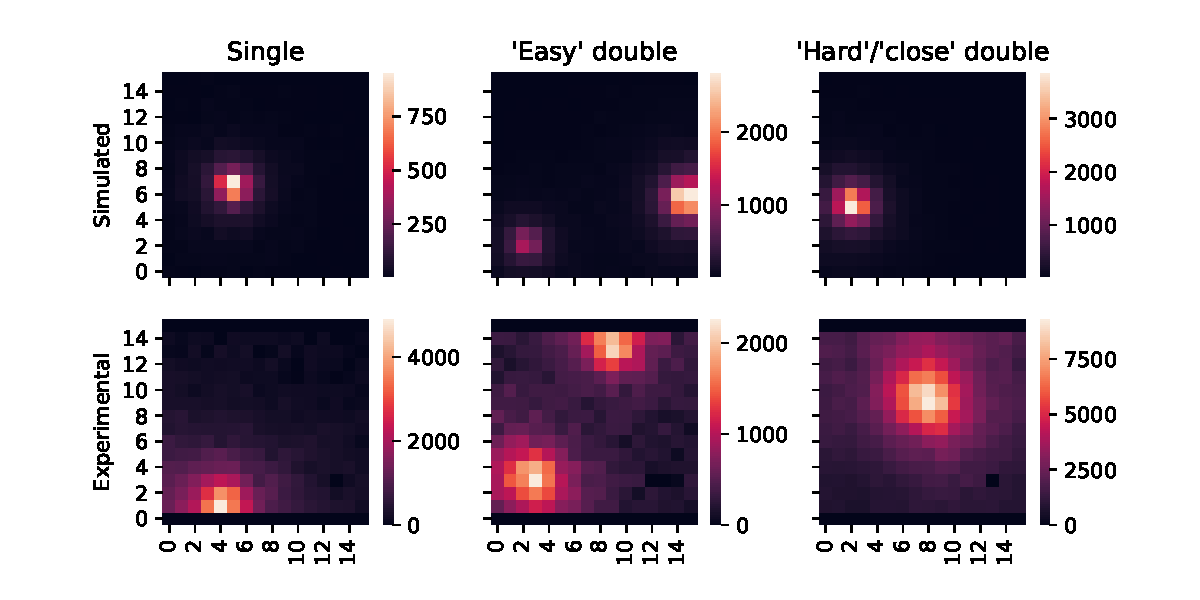
\includegraphics[width=\textwidth]{chapters/theory/figures/detector_image_samples.pdf}
    \caption{\label{fig:exp-background-sample-images} Sample images from 
    simulated and experimental datasets. The top row contains simulated samples
    and the bottom row contains experimental samples. The labeling as "easy" and "hard"
    double events is based on experience from hand-labeling, and theoretical
    expectations.}
\end{figure}
Simulated data is generated using GEANT4 \cite{Agostinelli2003}, and contains
two million simulated single and double events, balanced at a 50/50 ratio. 
Positions of origin are uniformly distributed in the detector image, and 
event energies are uniformly distributed between 0 to 1MeV. Pixel intensities 
range from 0 to 10000.

The experimental data is taken from a recent beta-decay experiment. This data differs
from the simulated data in some ways:
\begin{itemize}
	\item The positions of events in the detector images are expected to follow a more
	gaussian distribution rather than the uniform distribution. This is due to the
	nature of the experiment and how the particle beam is formed.
	\item Energy fluctuations in the scintillator makes experimental data look more
	'noisy' than simulated data.
	\item The ratio of single events to double events is not expected to be balanced.
	Rather, we expect to see a much larger amount of single events than double events.
	\item Some pixels in the experimental detector images will be set to zero if that
	pixel exhibits erratic behaviour. For some specific pixels this is true for the
	entire dataset. These pixels are the entire rows 0 and 15, plus pixel (13,3).
\end{itemize}
In our analysis of experimental data, we use two datasets. One set of 260147 decay events from a beta-decay
experiments, and one set of 100000 decay events where we have two additional energy-related
attributes available. These are DDAS\cite{msu-ddas}-energies and fit-energies. 
Both are measured using the PSPMT dynode signal. The DDAS energy is the energy
provided by the onboard signal processing algorithms of the DDAS system.
It is determined from the digitized detector signal using a trapezoidal filter.
The fit energy is determined offline by analyzing digitized detector signals.
The detector signal is modelled using a constant baseline plus a logistic rise 
convoluted with an exponential decay. This model signal is fit to the recorded
pulse using standard nonlinear regression methods, and the fit energy is given by the
amplitude of the best fit to the recorded detector signal.

The relationship between the arbitrary energy values determined by DDAS or the fitting and 
real energies define a set of calibration parameters which can be compared to calibration 
parameters determined using source data. Ideally, the calibration parameters determined using
machine learning models and the calibration parameters determined using source data should 
be the same or similar. 

\subsection{Simulated datasets}\label{sec:experimental-background-data-sim}
To explore the effect of some properties found in the experimental data, we
make three simulated datasets. The first (a) without any modifications.
The second (b) is designed to monitor the effects occurrences of 'dead' pixels in 
experimental data may have on model performance. When a pixel is unresponsive or 
displays otherwise erratic behaviour, the value of that pixel is set to zero in the 
given detector image. For some select pixels, this is the case for the entire dataset. 
The pixels are the entire top and bottom rows, and the pixel located at (13,3) when viewing 
an image as a 16x16 x,y-grid.
The third dataset (c) is designed to monitor any possible bias imposed on the models when trained
on a balanced dataset. As mentioned above, the expectation is that experimental data largely
consists of single decays, with double decays being much more of a rarity. When training a model
on a balanced dataset, we may impose a bias towards predicting a somewhat balanced amount of
each class. Intentionally reducing the presence of one class in the dataset may provide some insight
into whether or not this happens. In this case, we attempt to approximate the experimental data by
reducing the presence of double decays to only ~5\% of the total number of decays.


\chapter{Method}
The programming language chosen for implementing experiments performed
in this thesis is Python. Python has quickly grown to become one of the
most popular languages overall, and especially in the machine learning community.
Together with its extensive amount of available libraries, it allows for
fast prototyping of solutions, and excellent readability. For machine learning
purposes there are several libraries commonly used in the natural sciences.
The code developed for data processing and analysis in the thesis is available in two
GitHub repositories:
\begin{itemize}
    \item \url{https://github.com/geirtul/master_analysis}
    contains scripts and notebooks used in analysis of the data, as well as trained
    models and experiment logs.
    \item \url{https://github.com/geirtul/master_scripts}
    contains an installable python module with data import scripts and various helper
    functions used by the analysis repository.
\end{itemize}
Additionally, for a briefer overview and introduction to analysis of beta-decay
data using machine learning we have made a smaller example repository available
at \url{https://github.com/geirtul/event_classification_example}. The choice to use
a version control system such as GitHub stems from one of science's fundamental
principles - reproducibility. The code is freely available for anyone to inspect and
use.

\section{TensorFlow}
The TensorFlow\cite{tensorflow2016} library is developed by Google, and is one of the most
used libraries for machine learning in Python. It allows for designing complex learning
algorithms efficiently, and also includes the Keras API\cite{keras2015}, allowing
easy-to-follow implementations of standard architectures and pipelines. Using this API,
with TensorFlow as the backend framework, we build and train all models in this thesis.

\section{Building and training a model}
Building a machine learning model using TensorFlow and Keras is a straightforward
process. By utilizing the \lstinline{Sequential} class, we can stack the desired layers
with given properties, and TensorFlow takes care of the rest.
\lstinputlisting[label={code:end-to-end-example}, caption={End-to-end example of building, training,
and evaluating a model.}]{chapters/theory/tensorflow_example.py}
An end-to-end example of how to build, train and evaluate a model using
a small sample of simulated data is shown in \ref{code:end-to-end-example}.

\section{Pretrained network and feature extraction}\label{sec:method-pretrained}
A common strategy when working with representation- or transfer learning,
is to use a \textit{pretrained} model. State-of-the-art (SOTA) models typically
require enormous hardware resources and considerable time to train,
but simply passing inputs through them without any backpropagation does not.
They are trained on millions of inputs, and we seek to exploit their ability to
generalize. The SOTA models serve as feature extractors, and we train our own,
more specialized models to make predictions from the extracted features.
Many such models are available through the Keras API, and we have used
parts of VGG16 \cite{Simonyan2015} as part of this feature extraction.
The steps involved are as follows:
\begin{itemize}
    \item Initialize a \lstinline{Sequential} model like shown in \ref{code:end-to-end-example}.
    \item Add an \lstinline{InputLayer} suited to our inputs to the model. In our case this is
    (16, 16, 3) because VGG16 is trained on RGB images. Our images only have one channel, but we 
    can create 'pseudo-channels' by concatenating our images along the last axis.
    \item Loop over layers in the pretrained VGG16 model, adding them one by one to
    our Sequential model until the maximum number of layers have been added.
    Due to \lstinline{MaxPooling2D} layers, which cut the size of the inputs to the
    next layer in half, the number of layers we can use is lower than the number of layers
    in the full VGG16 model.
    \item Set each extracted layer's \textit{trainable} attribute to False. We don't want
    to adjust weights in this large, complex network.
    \item Add a \lstinline{Flatten} layer, which creates a one-dimensional vector of the
    extracted features.
    \item Add a desired number of \lstinline{Dense} layers to build a top-level network
    which will take the extracted features as input.
\end{itemize}
We are essentially treating the SOTA model's layers as a good initialization for our
final model.

\section{Data separation}
Separating our data into two sets with no overlap allows us to make an estimate of
our models' performance in the real world, on so-called 'out-of-sample' data.
This relates closely to the concepts of over- and underfitting. Neither the models,
nor ourselves, will see the split off dataset until all optimization and training
is completed. This way, leakage of information from what should be the out-of-sample
dataset is prevented, and a better performance estimate is reached. In this thesis we
use three terms for datasets - training, validation, and test. The test set is the data
which is hidden away until we have done all we can to optimize our models.
The training data is the rest, which when split into K folds for cross-validation
serves as $K-1$ folds of training data, and 1 fold as vaildation data.
\chapter{Results}
\noindent The first task we face is whether or not we can use machine learning algorithms to 
separate two types of events in a simulated nuclear physics dataset. This being possible
is the minimum requirement a model must meet if we are to apply it to experimental data.
We present the results of training five different models on three simulated 
datasets, as described in section \ref{sec:experimental-background-data}).
Performance is measured using the $F1$ score and confusion matrix. The models range from
the simple logistic regressor, to a deeper CNN architecture with multiple layers. Additionally,
we include a model based on VGG16, as outlined in section \ref{section:method-pretrained},
fine-tuned on simulated data. Somewhat separate from classification, our second objective
is predicting positions of origin and energies associated with events in the dataset.
We follow the same strategy as for classification, with the logistic model replaced by a linear
regressor. The same minimum requirement is valid for regression - models trained on simulated data
must be able to make reasonable predictions. By 'reasonable' we mean 'better than random guessing'.
For this task the performance is measured using the $R2$ score. The variability in results is 
estimated using a K-fold cross-validation approach, with $K = 5$ \cite{Stone1974}.
As a quick recap, the three simulated datasets mentioned are:
\begin{enumerate}[a)]
    \item No changes.
    \item Select pixels set to zero throughout the dataset.
    \item Select pixels set to zero throughout the data, and imbalanced number of single
    and double decays (reduced amount of double decays).
\end{enumerate}

\noindent The machine learning experiments conducted in this thesis were performed
using the AI-Hub computational cluster at the University of Oslo. This resource 
consists of three machines with four RTX 2080 Nvidia GPU’s (graphics
processing unit) each. These cards have ~10GB of memory available for the
allocation of models.

\section{Preliminary analysis}
We begin by looking into the simulated data, more specifically looking for correlations
in the energies and pixel intensities. Note that these results are generated using
dataset (a). In figure \ref{fig:simulated_corrcoeff} we show
the correlation matrix for simulated single and double decays. For single decays, there
is a strong correlation between the energy of the event, the sum of intensities in an image,
and also between the event energy and the intensity of the highest intensity pixel.
The correlation matrix for double events shows similar results. The same, strong correlation
is found for $E1 + E2$ in double decays as for $E1$ in single decays. That is, the total energy
in an event is strongly correlated with the total intensity of pixels in the image.
\begin{figure}
\centering
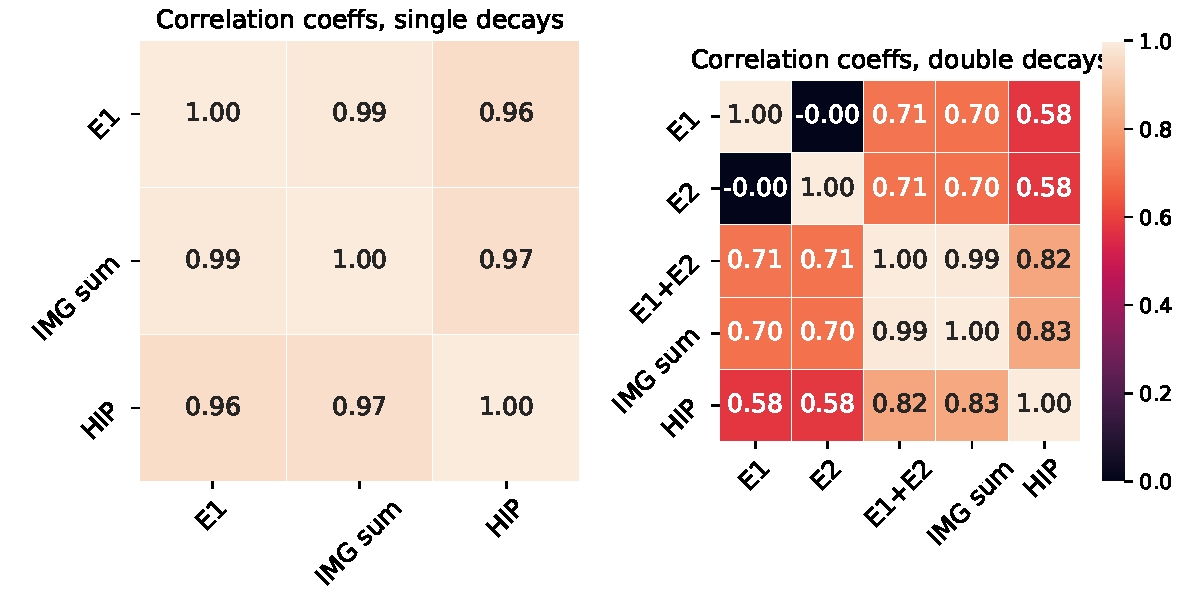
\includegraphics[width=\textwidth]{chapters/results/figures/simulated_corrcoeff.pdf}
\caption{\label{fig:simulated_corrcoeff}Correlation matrices for simulated data,
    separated into single and double decays. $E1$ and $E2$ are the energies corresponding
    to event 1 and event 2 in simulated data. For single events there is no event 2.
    $Sum(image)$ is the sum of all intensities per image in the dataset. HIP is short for
    Highest Intensity Pixel value.
    }
\end{figure}


\noindent Next, we investigate some directly comparable quantities shared by simulated and
experimental data. The distributions of total intensity and highest intensity pixels
in images are shown in figure \ref{fig:comparison-intensity}. 
\begin{figure}
\centering
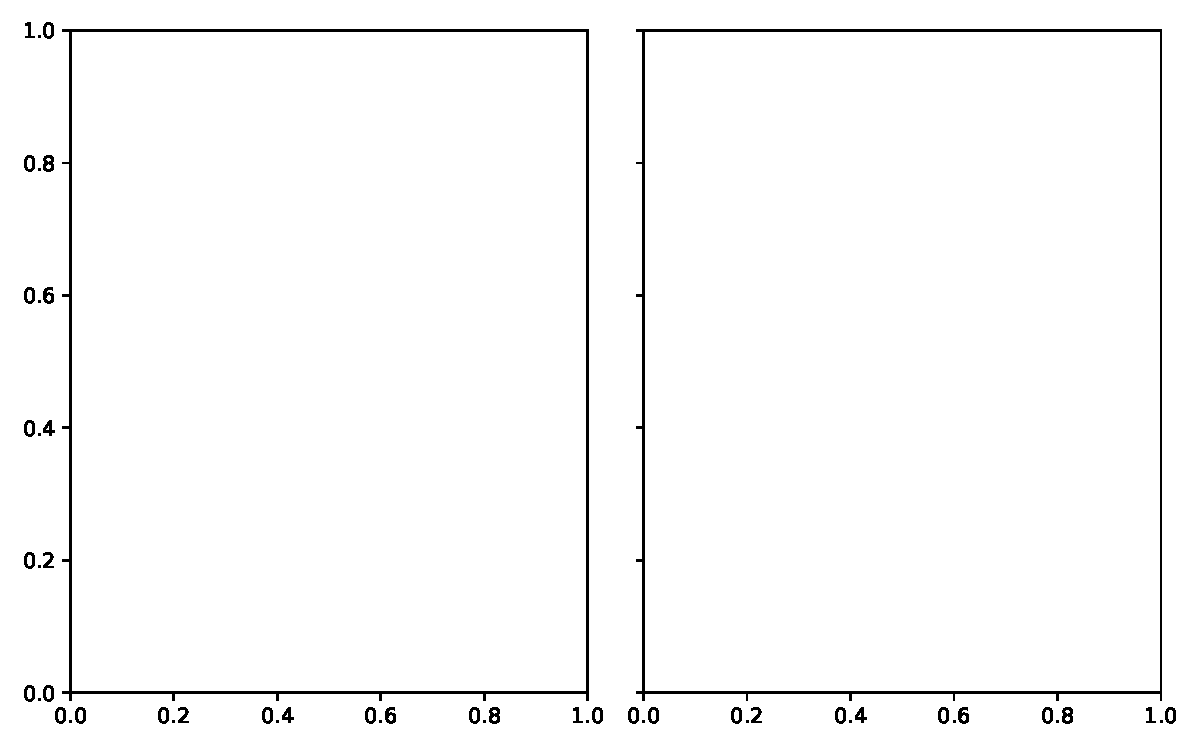
\includegraphics[width=\textwidth]{chapters/results/figures/comparison_intensity.pdf}
\caption{\label{fig:comparison-intensity}Distributions of total pixel intensities and
highest intensities in experimental and simulated decays. Top row compares experimental 
decays and all simulated decays. The bottom row shows the same distributions, but with simulated
decays split into single and double events. The calculations are done post normalization, so
the maximum possible intensity is 1.0.}
\end{figure}
\noindent To relate these distributions more closely to the models themselves, 
the distributions are generated after normalization of the
images. As such, these distributions are what the models 'see'. Looking to the top left
in figure \ref{fig:comparison-intensity} there are a fairly large amount of experimental
decays with higher total intensity than what is present in the simulated data. In the bottom
left plot, it is also clear that there is a point where simulated single and double decays no longer
overlap in total intensities. For the right-hand plots of highest intensity values, there is no such
clear difference between the datasets.
To provide another point of view for this difference, we plot the total intensity in images as
a function of the highest intensity in the images. 
The plot is shown in figure \ref{fig:intensity-hip-comparison}, along with linear fits to the
data.
\begin{figure}
\centering
\includegraphics[width=\textwidth]{chapters/results/figures/intensity_hip_comparison.pdf}
\caption{\label{fig:intensity-hip-comparison}Scatterplot of sum of intensities in images vs
the highest intensity in the same image, for both experimental and simulated decays.
Linear fits give slopes of $a_{experimental}=36.05$ and $a_{simulated}=11.69$.}
\end{figure}
\noindent There is a clear difference between the datasets in that the experimental data
has a higher total intensity. We will come back to these results as we review model
performance on experimental data.

\section{Classification}
\subsection{Classification on simulated data}
In table \ref{tab:classification-simulated-all-f1-auc} the performance of each model
is reported through the estimated $F1$-score, for each of the datasets. 
\begin{table}
\centering
\caption{
Test set F1-scores and roc-AUC scores for classification of simulated datausing multiple models.
Models are trained on a) unmodified data, b) data where specific pixels are set to zero to mimic
'dead' pixels in experimental data, and c) same as b) and imbalanced to mimic experimental data. 
Error estimates are the standard deviation in results from k-fold cross-validation with $K=5$ folds.
}
\label{tab:classification-simulated-all-f1-auc}
\begin{tabular}{llllll}
\toprule
{} &                                            Logistic &                                               Dense &                                       Convolutional &                                    Pretrained VGG16 &                                              Custom \\
\midrule
F1-score (a) &  $\underset{\num{+- 7.727e-03 }  }{\num{ 0.738 } }$ &  $\underset{\num{+- 1.329e-02 }  }{\num{ 0.91 } }$ &  $\underset{\num{+- 6.286e-03 }  }{\num{ 0.964 } }$ &  $\underset{\num{+- 1.591e-02 }  }{\num{ 0.911 } }$ &  $\underset{\num{+- 2.260e-02 }  }{\num{ 0.957 } }$ \\
F1-score (b) &  $\underset{\num{+- 2.273e-03 }  }{\num{ 0.732 } }$ &  $\underset{\num{+- 8.276e-03 }  }{\num{ 0.916 } }$ &  $\underset{\num{+- 3.640e-02 }  }{\num{ 0.758 } }$ &  $\underset{\num{+- 1.926e-02 }  }{\num{ 0.897 } }$ &  $\underset{\num{+- 7.601e-03 }  }{\num{ 0.938 } }$ \\
F1-score (c) &  $\underset{\num{+- 8.483e-02 }  }{\num{ 0.292 } }$ &  $\underset{\num{+- 1.233e-01 }  }{\num{ 0.52 } }$ &  $\underset{\num{+- 9.458e-02 }  }{\num{ 0.9 } }$ &  $\underset{\num{+- 3.606e-02 }  }{\num{ 0.823 } }$ &  $\underset{\num{+- 1.047e-01 }  }{\num{ 0.97 } }$ \\
AUC (a)      &  $\underset{\num{+- 6.515e-04 }  }{\num{ 0.832 } }$ &  $\underset{\num{+- 1.774e-02 }  }{\num{ 0.956 } }$ &  $\underset{\num{+- 2.185e-03 }  }{\num{ 0.988 } }$ &  $\underset{\num{+- 8.505e-03 }  }{\num{ 0.956 } }$ &  $\underset{\num{+- 2.218e-02 }  }{\num{ 0.979 } }$ \\
AUC (b)      &  $\underset{\num{+- 9.779e-04 }  }{\num{ 0.832 } }$ &  $\underset{\num{+- 2.604e-03 }  }{\num{ 0.956 } }$ &  $\underset{\num{+- 9.848e-03 }  }{\num{ 0.977 } }$ &  $\underset{\num{+- 9.530e-03 }  }{\num{ 0.949 } }$ &  $\underset{\num{+- 1.763e-03 }  }{\num{ 0.99 } }$ \\
AUC (c)      &  $\underset{\num{+- 1.601e-03 }  }{\num{ 0.832 } }$ &  $\underset{\num{+- 2.750e-03 }  }{\num{ 0.83 } }$ &  $\underset{\num{+- 8.035e-03 }  }{\num{ 0.944 } }$ &  $\underset{\num{+- 4.376e-03 }  }{\num{ 0.92 } }$ &  $\underset{\num{+- 5.312e-04 }  }{\num{ 0.986 } }$ \\
\bottomrule
\end{tabular}
\end{table}

As a benchmark for transfer learning, we are including a model based on a state of the art pretrained 
network\cite{Simonyan2015}, as outlined in section \ref{sec:method-pretrained}. 
In in figure \ref{fig:confmat-simulated}, we show the confusion matrix for prediction
on test set data for all the models, including normalized values for each event type.
\begin{figure}
\centering
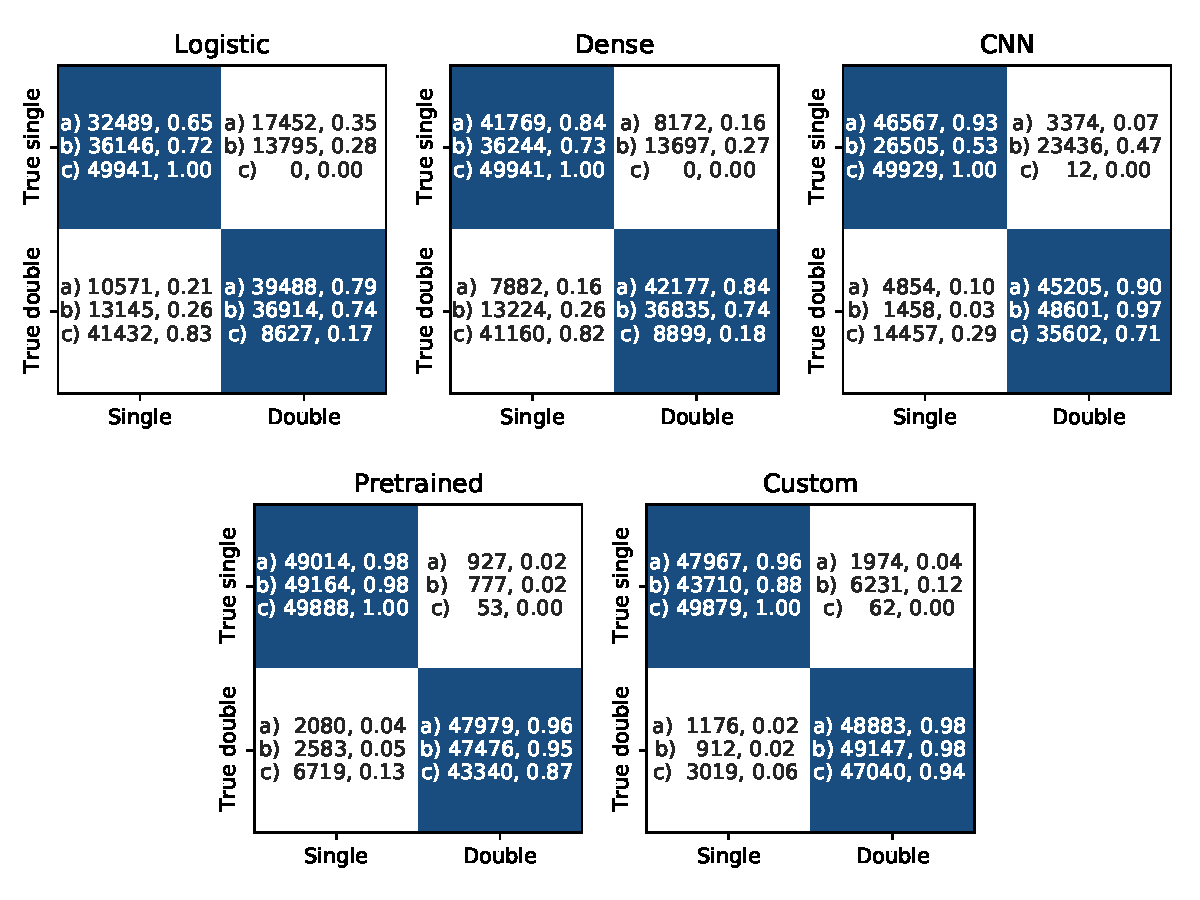
\includegraphics[width=\textwidth]{chapters/results/figures/confmat_simulated.pdf}
\caption{\label{fig:confmat-simulated}Confusion matrices for each model trained
on simulated data. For each model and dataset, the number of events and ratio of each
event type are given. a) unmodified data. b) select pixels set to zero. c) Same as in b)
with the intentionally imbalanced.}
\end{figure}. The F1-scores show decreasing
performance for most models when applying modifications to the unmodified simulated dataset.
When training on an intentionally imbalanced dataset the models without CNN architectures 
show a steep decrease in performance.
Considering the confusion matrix we see that the logistic regressor and dense network
suffer from predicting mostly every sample to be single events. Looking back to the
$F1$-scores again, there is not a significant increase in performance between the
CNN and the Custom model on unmodified data, but the custom model performs strongly
across all datasets, with a low amount of misclassified events relative to the other
models. Again looking at the confusion matrices (figure \ref{fig:confmat-simulated}),
Double decays are more often misclassified as single than the opposite.
Next, we apply the 'classifiers' to experimental data.

\subsection{Classification on experimental data}
Classification of experimental data poses a different set of challenges when it comes
to evaluating our results. We currently only have a small number of events that are
hand labelled as double events, which may be used as a form of verification. As mentioned in section
\ref{sec:experimental-background}, we expect the number of double events in the experimental
data to be much lower than single events. Inspecting the ratio of predicted singles to predicted
doubles can then be an initial indication of how a model is performing. It is, however,
not conclusive. Correctly classified hand labelled events are another indication, but
is also not conclusive. In table \ref{tab:classification-experimental-ratios}, the ratios
of predicted singles to predicted doubles are presented for each model trained on each
dataset. The actual number of predictions for each class are included below the ratios.
\begin{table}
\centering
\caption{
Decay event classification on experimental data, with models trained on:
a) unmodified data, b) data where specific pixels are set to zero to mimic
'dead' pixels in experimental data, and c) same as b) and imbalanced to mimic experimental data.
}
\label{tab:classification-experimental-ratios}
\begin{tabular}{lllllll}
\toprule
{} &                                     Single (a) &                                     Double (a) &                                     Single (b) &                                     Double (b) &                                     Single (c) &                                     Double (c) \\
\midrule
Logistic   &  $\underset{\num{ 198210 }  }{\num{ 0.762 } }$ &  $\underset{\num{ 61937 }  }{\num{ 0.238 } }$ &  $\underset{\num{ 202426 }  }{\num{ 0.778 } }$ &  $\underset{\num{ 57721 }  }{\num{ 0.222 } }$ &  $\underset{\num{ 260145 }  }{\num{ 1.000 } }$ &  $\underset{\num{ 2 }  }{\num{ 0.000 } }$ \\
Dense      &  $\underset{\num{ 97487 }  }{\num{ 0.375 } }$ &  $\underset{\num{ 162660 }  }{\num{ 0.625 } }$ &  $\underset{\num{ 100778 }  }{\num{ 0.387 } }$ &  $\underset{\num{ 159369 }  }{\num{ 0.613 } }$ &  $\underset{\num{ 260122 }  }{\num{ 1.000 } }$ &  $\underset{\num{ 25 }  }{\num{ 0.000 } }$ \\
CNN        &  $\underset{\num{ 63051 }  }{\num{ 0.242 } }$ &  $\underset{\num{ 197096 }  }{\num{ 0.758 } }$ &  $\underset{\num{ 66790 }  }{\num{ 0.257 } }$ &  $\underset{\num{ 193357 }  }{\num{ 0.743 } }$ &  $\underset{\num{ 98594 }  }{\num{ 0.379 } }$ &  $\underset{\num{ 161553 }  }{\num{ 0.621 } }$ \\
Pretrained &  $\underset{\num{ 138614 }  }{\num{ 0.533 } }$ &  $\underset{\num{ 121533 }  }{\num{ 0.467 } }$ &  $\underset{\num{ 137765 }  }{\num{ 0.530 } }$ &  $\underset{\num{ 122382 }  }{\num{ 0.470 } }$ &  $\underset{\num{ 259448 }  }{\num{ 0.997 } }$ &  $\underset{\num{ 699 }  }{\num{ 0.003 } }$ \\
Custom     &  $\underset{\num{ 26277 }  }{\num{ 0.101 } }$ &  $\underset{\num{ 233870 }  }{\num{ 0.899 } }$ &  $\underset{\num{ 24738 }  }{\num{ 0.095 } }$ &  $\underset{\num{ 235409 }  }{\num{ 0.905 } }$ &  $\underset{\num{ 52951 }  }{\num{ 0.204 } }$ &  $\underset{\num{ 207196 }  }{\num{ 0.796 } }$ \\
\bottomrule
\end{tabular}
\end{table}

Overall there is a strong preference for classifying events as double decays. This makes
the validation using hand labelled doubles in table \ref{tab:classification-experimental-labeled-doubles}
somewhat moot, since it is hard to attribute these 'correct' classifications to the models'
ability to recognize the double decays.
\begin{table}
\centering
\caption{
Decay event classification on 17 labeled samples of experimental data. The 17 samples are all
labeled as double events. Models are trained on simulated data with a varying degree of modification:
a) unmodified data, b) data where specific pixels are set to zero to mimic
'dead' pixels in experimental data, and c) same as b) and imbalanced to mimic experimental data.
The numbers are shown as the normalized ratio of predicted event type, with the actual amount of
events predicted of that type below.
}
\label{tab:classification-experimental-labeled-doubles}
\begin{tabular}{lllllll}
\toprule
{} &                                Single (a) &                                 Double (a) &                                Single (b) &                                 Double (b) &                                Single (c) &                                 Double (c) \\
\midrule
Logistic   &  $\underset{\num{ 0 }  }{\num{ 0.000 } }$ &  $\underset{\num{ 17 }  }{\num{ 1.000 } }$ &  $\underset{\num{ 0 }  }{\num{ 0.000 } }$ &  $\underset{\num{ 17 }  }{\num{ 1.000 } }$ &  $\underset{\num{ 1 }  }{\num{ 0.059 } }$ &  $\underset{\num{ 16 }  }{\num{ 0.941 } }$ \\
Dense      &  $\underset{\num{ 0 }  }{\num{ 0.000 } }$ &  $\underset{\num{ 17 }  }{\num{ 1.000 } }$ &  $\underset{\num{ 0 }  }{\num{ 0.000 } }$ &  $\underset{\num{ 17 }  }{\num{ 1.000 } }$ &  $\underset{\num{ 0 }  }{\num{ 0.000 } }$ &  $\underset{\num{ 17 }  }{\num{ 1.000 } }$ \\
CNN        &  $\underset{\num{ 0 }  }{\num{ 0.000 } }$ &  $\underset{\num{ 17 }  }{\num{ 1.000 } }$ &  $\underset{\num{ 0 }  }{\num{ 0.000 } }$ &  $\underset{\num{ 17 }  }{\num{ 1.000 } }$ &  $\underset{\num{ 0 }  }{\num{ 0.000 } }$ &  $\underset{\num{ 17 }  }{\num{ 1.000 } }$ \\
Pretrained &  $\underset{\num{ 0 }  }{\num{ 0.000 } }$ &  $\underset{\num{ 17 }  }{\num{ 1.000 } }$ &  $\underset{\num{ 0 }  }{\num{ 0.000 } }$ &  $\underset{\num{ 17 }  }{\num{ 1.000 } }$ &  $\underset{\num{ 3 }  }{\num{ 0.176 } }$ &  $\underset{\num{ 14 }  }{\num{ 0.824 } }$ \\
Custom     &  $\underset{\num{ 0 }  }{\num{ 0.000 } }$ &  $\underset{\num{ 17 }  }{\num{ 1.000 } }$ &  $\underset{\num{ 0 }  }{\num{ 0.000 } }$ &  $\underset{\num{ 17 }  }{\num{ 1.000 } }$ &  $\underset{\num{ 0 }  }{\num{ 0.000 } }$ &  $\underset{\num{ 17 }  }{\num{ 1.000 } }$ \\
\bottomrule
\end{tabular}
\end{table}

\begin{figure}
\centering
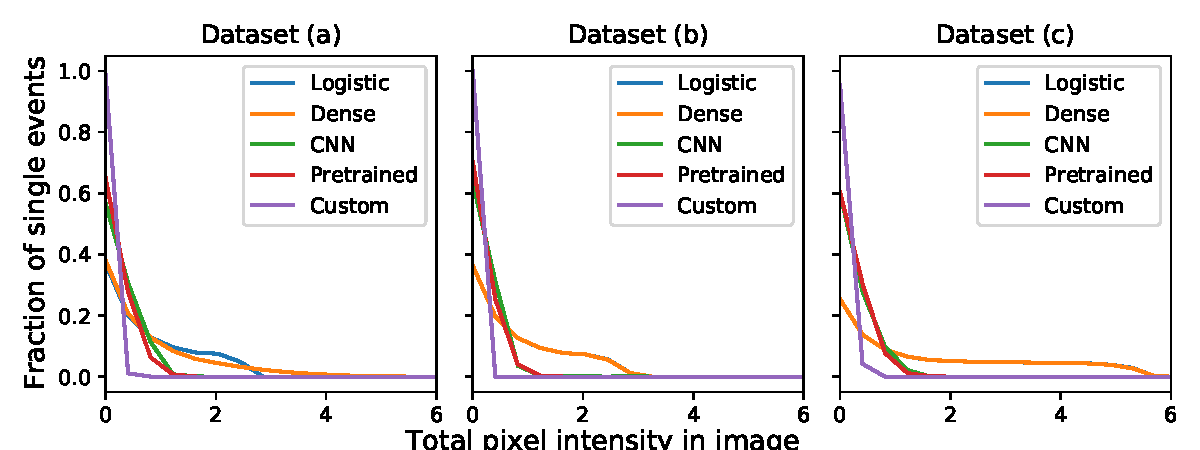
\includegraphics[width=\textwidth]{chapters/results/figures/classification_experimental_single_fractions.pdf}
\caption{\label{fig:experimental-single-fractions}Fraction of predicted singles as a function of
total intensity in images, for each model trained on simulated data.  a) unmodified data. b) select pixels set to zero. 
c) Same as in b) with the intentionally imbalanced.}
\end{figure}
As the number of events is large, manual inspection of each predicted class is not feasible.
In figure \ref{fig:experimental-single-fractions} we show the fraction of predicted single events
in experimental data as a function of total intensity in each image. Regardless of which simulated
dataset a model is trained on, the majority of  single events are predicted at low total intensites.
The only exception to this is the Dense model trained on dataset $c$. Keep in mind, however, that the
total intensities for experimental data span from 0 to ~18 (see figure \ref{fig:comparison-intensity}).
To further prod this apparent trend, we perform a simple test using the Custom model trained on dataset $b$.
For a set of single events for which we know the model has good performance, we multiply the image intensities
with a scaling factor from 0-10. The aim is to see the effect of increasing total intensity in
images on the classification accuracy. The result is shown in figure \ref{fig:simulated-scaled-intensities}.
\begin{figure}
\centering
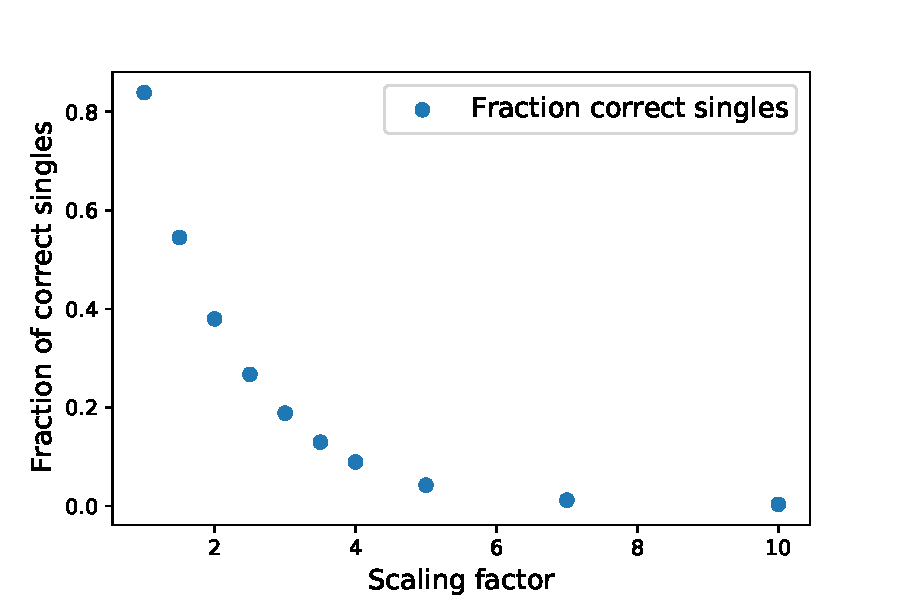
\includegraphics[width=\textwidth]{chapters/results/figures/simulated_scaled_intensity.pdf}
\caption{\label{fig:simulated-scaled-intensities}Fraction of simulated single events correctly classified
as a function of scaling factor used to increase the total intensity in simulated
decays. The model used for classification is the Custom model trained on dataset (b),
which has select pixels set to zero.}
\end{figure}
From this figure, there is a clear trend towards a lower fraction of events correctly classified as single 
decays when the intensities in images increases. Note that at a scaling factor of 4 the total intensities in
the simulated images approach the highest total intensities in the experimental decay data.
 
\section{Regression}
Assuming data has already been classified, we aim to predict the energy of the decays and their
position of origin. Because there is a travel distance between the 
ejection site and the point the energy is deposited, the positions aren't necessarily
the locations of the highest-intensity pixels in the detector images. Our hypothesis is
then that there are sufficient structures and spacial relationships in the detector images to
allow a model to determine these positions.
Note that for regression the models are trained on single or double events exclusively.
A consequence of this is that for dataset $c$ the set of single events is
identical to that of set $b$, causing near-identical results between these two sets.

\subsection{Position of origin}
In table \ref{tab:regression-simulated-all-positions-r2} the R2-scores for all models
trained on simulated data are presented.
\begin{table}
\centering
\caption{
Test set R2-scores for regression of positions of origin on simulated data, with models trained on data with: 
a) no modifications, b) specific pixels set to zero to mimic experimental data, and c) imbalanced dataset
in addition to modifications in b) to further mimic experimental data. Error estimates are the standard deviation 
in results from validation data in k-fold cross-validation with $K=5$ folds.
}
\label{tab:regression-simulated-all-positions-r2}
\begin{tabular}{llllll}
\toprule
{} &                                              Linear &                                               Dense &                                                 CNN &                                           Pretrained &                                              Custom \\
\midrule
Single (a) &  $\underset{\num{+- 2.889e-03 }  }{\num{ 0.8 } }$ &  $\underset{\num{+- 7.007e-04 }  }{\num{ 0.988 } }$ &  $\underset{\num{+- 9.207e-04 }  }{\num{ 0.997 } }$ &  $\underset{\num{+- 2.229e-01 }  }{\num{ 0.997 } }$ &  $\underset{\num{+- 1.366e-04 }  }{\num{ 0.999 } }$ \\
Single (b) &  $\underset{\num{+- 2.749e-03 }  }{\num{ 0.781 } }$ &  $\underset{\num{+- 1.406e-03 }  }{\num{ 0.982 } }$ &  $\underset{\num{+- 1.110e-03 }  }{\num{ 0.98 } }$ &  $\underset{\num{+- 4.513e-04 }  }{\num{ 0.997 } }$ &  $\underset{\num{+- 9.603e-04 }  }{\num{ 0.995 } }$ \\
Single (c) &  $\underset{\num{+- 2.749e-03 }  }{\num{ 0.781 } }$ &  $\underset{\num{+- 1.424e-03 }  }{\num{ 0.982 } }$ &  $\underset{\num{+- 1.080e-03 }  }{\num{ 0.98 } }$ &  $\underset{\num{+- 4.932e-04 }  }{\num{ 0.997 } }$ &  $\underset{\num{+- 1.639e-03 }  }{\num{ 0.993 } }$ \\
Double (a) &  $\underset{\num{+- 3.766e-03 }  }{\num{ 0.37 } }$ &  $\underset{\num{+- 5.601e-03 }  }{\num{ 0.456 } }$ &  $\underset{\num{+- 1.603e-03 }  }{\num{ 0.471 } }$ &  $\underset{\num{+- 1.552e-01 }  }{\num{ 0.29 } }$ &  $\underset{\num{+- 3.467e-04 }  }{\num{ 0.493 } }$ \\
Double (b) &  $\underset{\num{+- 6.815e-04 }  }{\num{ 0.364 } }$ &  $\underset{\num{+- 3.431e-03 }  }{\num{ 0.458 } }$ &  $\underset{\num{+- 1.835e-03 }  }{\num{ 0.435 } }$ &  $\underset{\num{+- 1.550e-01 }  }{\num{ 0.289 } }$ &  $\underset{\num{+- 2.865e-04 }  }{\num{ 0.489 } }$ \\
Double (c) &  $\underset{\num{+- 7.768e-03 }  }{\num{ 0.357 } }$ &  $\underset{\num{+- 9.456e-03 }  }{\num{ 0.417 } }$ &  $\underset{\num{+- 2.507e-03 }  }{\num{ 0.442 } }$ &  $\underset{\num{+- 8.452e-01 }  }{\num{ -0.924 } }$ &  $\underset{\num{+- 4.187e-03 }  }{\num{ 0.478 } }$ \\
\bottomrule
\end{tabular}
\end{table}

\noindent A similar trend as was seen for classification
can be observed for single events, where models are trained on unmodified data. Even
a linear regressor predicts positions of origin fairly well, but it is clear
that the neural networks perform at a much higher level in this case. They have strong
R2-scores of 0.99 and higher, and very little degradation in performance with added 
modifications to the training data. Again, as with classification, the custom model
performs strongly across all datasets for single events, with the lowest variability across
experiments. However, in this regression task, the pretrained model.
In the case of regression on double events, none of the models accurately
predict positions of origins for both events.
\begin{table}
\centering
\caption{
Mean distances of predicted position of origin on experimental data, to center of highest intensity pixel (HIP).Models 
trained on data with: a) no modifications, b) specific pixels set to zero to mimic experimental data, and c) imbalanced dataset
in addition to modifications in b) to further mimic experimental data.
}
\label{tab:regression-experimental-dist-means}
\begin{tabular}{ll}
\toprule
{} & Mean distance [mm] \\
\midrule
LinReg (a)     &  $\num{ 19.19 }$ \\
Dense (a)      &  $\num{ 63.27 }$ \\
CNN (a)        &  $\num{ 10.72 }$ \\
Pretrained (a) &  $\num{ 17.52 }$ \\
Custom (a)     &  $\num{ 13.23 }$ \\
LinReg (b)     &  $\num{ 19.97 }$ \\
Dense (b)      &  $\num{ 32.06 }$ \\
CNN (b)        &  $\num{ 11.92 }$ \\
Pretrained (b) &  $\num{ 16.43 }$ \\
Custom (b)     &  $\num{ 4.39 }$ \\
LinReg (c)     &  $\num{ 19.97 }$ \\
Dense (c)      &  $\num{ 32.04 }$ \\
CNN (c)        &  $\num{ 11.85 }$ \\
Pretrained (c) &  $\num{ 16.43 }$ \\
Custom (c)     &  $\num{ 7.08 }$ \\
\bottomrule
\end{tabular}
\end{table}

In the absence of true positions for experimental decays, we rely on other
ways to estimate how regression models perform.
In figure \ref{fig:experimental-pos-dist} we look at how the predicted positions
are distributed around the highest intensity pixel in each experimental decay event.
As a comparison, we plot the same distribution using true values for positions in
simulated single decay events. We can see that the distributions overlap quite well
up until their respective peaks. Predictions on experimental decays have a wider
distribution than the target data, but as we've seen in the classification results this
difference in distributions is not a unique case.

\subsubsection{Energy}
In table \ref{tab:regression-simulated-all-energies-r2} we show the R2-scores for all
models trained on simulated data.
Performance when predicting single energies is across the board lower than what we saw
for positions of origin. On unmodified data, the models are to a large degree able to
predict energies, with R2-scores of 0.93 and above. For the modified datasets the CNN
suffers greatly and isn't able to account for variances in the data at all. Other models
see a less severe effect, but still a clear reduction in goodness of fit.
As was the case with the prediction of positions, no models predict energies
of double events with any useful degree of accuracy.
\begin{table}
\centering
\caption{
Test set R2-scores for regression of energies on simulated data, with models trained on data with: 
a) no modifications, b) specific pixels set to zero to mimic experimental data, and c) imbalanced dataset
in addition to modifications in b) to further mimic experimental data. Error estimates are the standard deviation 
in results from validation data in k-fold cross-validation with $K=5$ folds.
}
\label{tab:regression-simulated-all-energies-r2}
\begin{tabular}{llllll}
\toprule
{} &                                              Linear &                                               Dense &                                                 CNN &                                          Pretrained &                                              Custom \\
\midrule
Single (a) &  $\underset{\num{+- 3.334e-02 }  }{\num{ 0.932 } }$ &  $\underset{\num{+- 3.623e-02 }  }{\num{ 0.934 } }$ &  $\underset{\num{+- 4.088e-02 }  }{\num{ 0.937 } }$ &  $\underset{\num{+- 3.761e-02 }  }{\num{ 0.926 } }$ &  $\underset{\num{+- 2.997e-02 }  }{\num{ 0.944 } }$ \\
Single (b) &  $\underset{\num{+- 2.459e-02 }  }{\num{ 0.768 } }$ &  $\underset{\num{+- 2.222e-02 }  }{\num{ 0.745 } }$ &  $\underset{\num{+- 2.575e-02 }  }{\num{ 0.48 } }$ &  $\underset{\num{+- 1.948e-02 }  }{\num{ 0.781 } }$ &  $\underset{\num{+- 3.167e-02 }  }{\num{ 0.752 } }$ \\
Single (c) &  $\underset{\num{+- 2.459e-02 }  }{\num{ 0.768 } }$ &  $\underset{\num{+- 2.223e-02 }  }{\num{ 0.745 } }$ &  $\underset{\num{+- 2.522e-02 }  }{\num{ 0.432 } }$ &  $\underset{\num{+- 1.955e-02 }  }{\num{ 0.781 } }$ &  $\underset{\num{+- 2.956e-02 }  }{\num{ 0.724 } }$ \\
Double (a) &  $\underset{\num{+- 3.349e-02 }  }{\num{ 0.49 } }$ &  $\underset{\num{+- 3.084e-02 }  }{\num{ 0.49 } }$ &  $\underset{\num{+- 4.130e-02 }  }{\num{ 0.488 } }$ &  $\underset{\num{+- 3.138e-02 }  }{\num{ 0.489 } }$ &  $\underset{\num{+- 3.618e-02 }  }{\num{ 0.491 } }$ \\
Double (b) &  $\underset{\num{+- 3.157e-03 }  }{\num{ 0.485 } }$ &  $\underset{\num{+- 2.347e-03 }  }{\num{ 0.487 } }$ &  $\underset{\num{+- 7.096e-03 }  }{\num{ 0.478 } }$ &  $\underset{\num{+- 4.508e-03 }  }{\num{ 0.489 } }$ &  $\underset{\num{+- 3.659e-03 }  }{\num{ 0.464 } }$ \\
Double (c) &  $\underset{\num{+- 4.611e-02 }  }{\num{ 0.434 } }$ &  $\underset{\num{+- 4.583e-02 }  }{\num{ 0.422 } }$ &  $\underset{\num{+- 4.554e-02 }  }{\num{ 0.446 } }$ &  $\underset{\num{+- 3.868e-02 }  }{\num{ 0.417 } }$ &  $\underset{\num{+- 4.802e-02 }  }{\num{ 0.401 } }$ \\
\bottomrule
\end{tabular}
\end{table}


Due to the poor performance of models trained on simulated double events, and the
expected low frequency of double events in the experimental data, we only apply models
trained on simulated single events.
\begin{figure}
\centering
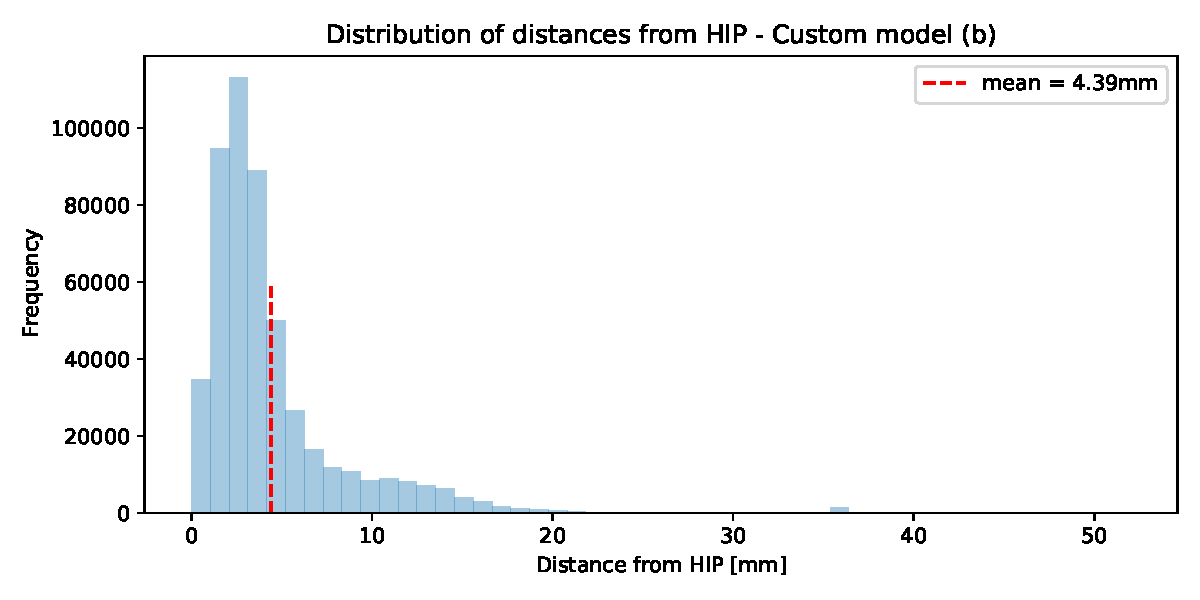
\includegraphics[width=\textwidth]{chapters/results/figures/experimental_pos_dist.pdf}
\caption{\label{fig:experimental-pos-dist} Distribution of distances between predicted
positions of origin and the highest intensity pixel(HIP) in the corresponding images. 
The model was a custom cnn architecture, trained on simulated data where (b) denotes 
that elect pixels were set to zero across the dataset. This model was selected for this
plot due to it having the lowest mean distance from HIP.}
\end{figure}

\chapter{Discussion}
\section{Classification}
With the goal of classifying experimental decay data, we set a minimum requirement
of first showing that machine learning algorithms can classify simulated decay events.
From the $F1$ scores shown in table \ref{tab:classification-simulated-all-f1-auc} we
can see that classification of simulated events is possible.
There is a clear performance gap between CNN-based architectures and the logistic regressor and dense
neural network. This gap may be expected, as CNN's are specifically designed for
machine learning involving images. Of the CNN architechtures, the deeper architectures
(Custom \ref{appendix:model-custom}, Pretrained \ref{appendix:model-pretrained}),
show less decrease in performance when trained on datasets with 'dead' pixels and
imbalanced representation of classes. When training models on an imbalanced dataset
these deeper models also appear less prone to simply classify most of events as one
class. In figure \ref{fig:confmat-simulated} we can see that this is the case for
the logistic and dense models.

With the ability to classify simulated events as either single or double decays,
we then applied the models trained on simulated data to experimental data.
Lacking true labels for experimental data, we look to other expecations, such
as the fraction of events predicted as single and double decays, shown in table
\ref{tab:classification-experimental-ratios}. Our expectation is that there is
a much larger amount of single decays present in experimental data than
double decays. In light of this expectation, the models' performance is not very good.
The models performing best on simulated data predict up to 90\% or more of the
experimental decays to be double decays. This is also the case for models trained
on dataset $c$ (imbalanced). In figure \ref{fig:comparison-intensity} we saw that
there is a difference in total intensity between simulated decays and experimental
decays. The experimental decays range higher in total intensity, and in figure
\ref{fig:intensity-hip-comparison} we also see that a higher maximum intensity in
an experimental event corresponds to a higher total intensity than for simulated
events. Additionally, the fraction of predicted single events as a function of total
intensity in images which we show in figure \ref{fig:experimental-single-fractions},
indicate that most single events are predicted for low total intensities in images.
In fact, single events are predicted almost exclusively in the region of total intensity
where single events are distributed in simulated data. We also concider the trend
of decreased fraction of correctly classified single decays in simulated data,
presented in figure \ref{fig:simulated-scaled-intensities}. Together,
this difference between simulated and experimental data may partially explain why a 
lot of events are classified as double decays. 

\section{Regression}
\subsection{Positions of origin}

\subsection{Energy}
With energies being closely correlated with total intensity in an image,
having dead pixels can be detrimental to the performance in predictions.
- show this somehow?
\chapter{Conclusion}
In this thesis, we have applied supervised machine learning algorithms to simulated and experimental
nuclear physics data. With the goal of leveraging the exact knowledge of properties in simulations to extract
vital patterns and representations, we trained models to classify simulated decay events as either 'single'
or 'double', and to predict the energy and positions of origin for events. To determine the effects of
some properties of the experimental data, we prepared additional simulated datasets where we incorporated
these properties. They were so-called 'dead' pixels in specific locations, and imbalanced class distribution.
We found that for simulated data a Convolutional Neural Network-based architecture is highly successful in the
classification of events across all the prepared datasets, with $F1$ scores up to $0.97$. 
This is not the case for the 'simpler' logistic and dense models, which suffer from the included properties 
in the datasets.
Classification on experimental data was not found to be successful, regardless of model performance on
simulated data. This may be partly explained by a difference in total intensity, or deposited energy,
between simulated and experimental data. We observe a trend across all models and training data, that
when classifying experimental decay events, most all event classified as single are in the lower
regime of total intensities. We observe the same trend if we classify simulated data where all pixel
intensities are scaled up.

We successfully trained models to predict positions of origin for simulated single decay events,
with $R2$ scores of $0.99$ and above for all simulated datasets. However, we were unable to
predict positions of origin for simulated double decay events with any degree of precision.
We found the same problem when predicting energies, and energy prediction was also sensitive
to the modifications in the data. A likely cause of this sensitivity may be the strong correlation
between energy and total pixel intensity in detector images, and the modifications effectively
acting as removal of information.

Without true positions for experimental data to directly test the models against,
making any strong conclusions for these results is hard. Proper verification of performance 
will have to wait until researchers can test the predicted positions on source data from the
experiment. However, we find that the positions predicted seem within reasonable limits, compared
with what is seen in simulated data. There is a risk that when the number of 'dead' pixels in a detector
image increases, the positions predicted may not be positions of the event itself, rather a position
based on the remaining information in the image.

We found similar results when predicting energies for experimental decays. Preliminary comparisons
with experimental calibration constants indicate that the predictions are not good on experimental
decays. The working theory is that the simulated training data predicts too many photons per unit
energy, resulting in the knowledge from simulated data not being transferable to the experimental
domain.

\section{Future work}
From the results found in this thesis, there may be grounds to adjust simulations based on
experimental data, or post-process the simulated datasets to better represent the experiment.
Another option could be to invest in hand labelling an experimental dataset which can be used
to tune the models used in this thesis. This could also allow for estimating upper and lower bounds
for the Receiver Operating Characteristic \ref{Claesen2015}, which we have not used in this thesis.
As the effect of pixels being set to zero value is detrimental to energy predictions, in particular,
efforts might be made to assess the magnitude of the effect, and whether or not it could be reasonable
to approximate pixel values. It may be worth looking into more traditional 2D peak-finding algorithms
for extracting 'obvious' double events in space. This could greatly speed up the process of generating a
labeled experimental dataset.

\bibliographystyle{mybibstyle}
\bibliography{library.bib}

\end{document}
